%% 
%% Copyright 2019-2020 Elsevier Ltd
%% 
%% This file is part of the 'CAS Bundle'.
%% --------------------------------------
%% 
%% It may be distributed under the conditions of the LaTeX Project Public
%% License, either version 1.2 of this license or (at your option) any
%% later version.  The latest version of this license is in
%%    http://www.latex-project.org/lppl.txt
%% and version 1.2 or later is part of all distributions of LaTeX
%% version 1999/12/01 or later.
%% 
%% The list of all files belonging to the 'CAS Bundle' is
%% given in the file `manifest.txt'.
%% 
%% Template article for cas-sc documentclass for 
%% double column output.

%\documentclass[a4paper,fleqn,longmktitle]{cas-sc}
\documentclass[a4paper,fleqn]{cas-sc}

% \usepackage[numbers]{natbib}
%\usepackage[authoryear]{natbib}
\usepackage[authoryear,longnamesfirst]{natbib}

%%%Author definitions
\def\tsc#1{\csdef{#1}{\textsc{\lowercase{#1}}\xspace}}
\tsc{WGM}
\tsc{QE}
\tsc{EP}
\tsc{PMS}
\tsc{BEC}
\tsc{DE}
%%%

% Uncomment and use as if needed
%\newtheorem{theorem}{Theorem}
%\newtheorem{lemma}[theorem]{Lemma}
%\newdefinition{rmk}{Remark}
%\newproof{pf}{Proof}
%\newproof{pot}{Proof of Theorem \ref{thm}}

% Auto-generated by sync_latex_results.py; do not edit by hand.
% Source: ALL_RESULTS_ORGANIZED_OLD_SPLIT_ROW4, corrected seed-13 40/10/50 split.
% Primary metric: macro boundary-relaxed containment F1 (macro_f1).

% Mean before/after scores over six skill views.
\providecommand{\BertSoftwareBefore}{\OURSREV{0.129}{0.128}}
\providecommand{\BertSoftwareAfter}{\OURSREV{0.592}{0.621}}
\providecommand{\BertSoftwareGain}{\OURSREV{0.462}{0.494}}
\providecommand{\BertJournalismBefore}{\OURSREV{0.174}{0.159}}
\providecommand{\BertJournalismAfter}{\OURSREV{0.643}{0.687}}
\providecommand{\BertJournalismGain}{\OURSREV{0.470}{0.529}}
\providecommand{\BertMergedBefore}{\OURSREV{0.151}{0.146}}
\providecommand{\BertMergedAfter}{\OURSREV{0.648}{0.670}}
\providecommand{\BertMergedGain}{\OURSREV{0.498}{0.524}}
\providecommand{\BartSoftwareBefore}{\OURSREV{0.050}{0.052}}
\providecommand{\BartSoftwareAfter}{\OURSREV{0.442}{0.489}}
\providecommand{\BartSoftwareGain}{\OURSREV{0.391}{0.438}}
\providecommand{\BartJournalismBefore}{\OURSREV{0.066}{0.062}}
\providecommand{\BartJournalismAfter}{\OURSREV{0.446}{0.476}}
\providecommand{\BartJournalismGain}{\OURSREV{0.380}{0.413}}
\providecommand{\BartMergedBefore}{\OURSREV{0.049}{0.055}}
\providecommand{\BartMergedAfter}{\OURSREV{0.499}{0.528}}
\providecommand{\BartMergedGain}{\OURSREV{0.449}{0.473}}
% Best evaluated configuration per domain.
\providecommand{\BestSoftwareModel}{prompted Gemini}
\providecommand{\BestSoftwareScore}{\OURSREV{0.654}{0.652}}
\providecommand{\BestSoftwarePrecision}{\OURSREV{0.669}{0.663}}
\providecommand{\BestSoftwareRecall}{\OURSREV{0.712}{0.706}}
\providecommand{\BestJournalismModel}{fine-tuned Swedish BERT}
\providecommand{\BestJournalismScore}{\OURSREV{0.643}{0.687}}
\providecommand{\BestJournalismPrecision}{\OURSREV{0.638}{0.601}}
\providecommand{\BestJournalismRecall}{\OURSREV{0.705}{0.872}}
\providecommand{\BestMergedModel}{fine-tuned Swedish BERT}
\providecommand{\BestMergedScore}{\OURSREV{0.648}{0.670}}
\providecommand{\BestMergedPrecision}{\OURSREV{0.626}{0.607}}
\providecommand{\BestMergedRecall}{\OURSREV{0.734}{0.824}}
% Evaluated configuration means over six skill views.
\providecommand{\BertSoftwareScore}{\OURSREV{0.592}{0.621}}
\providecommand{\BartSoftwareScore}{\OURSREV{0.442}{0.489}}
\providecommand{\GptSoftwareScore}{\OURSREV{0.617}{0.620}}
\providecommand{\ClaudeSoftwareScore}{\OURSREV{0.638}{0.637}}
\providecommand{\GeminiSoftwareScore}{\OURSREV{0.654}{0.652}}
\providecommand{\BertJournalismScore}{\OURSREV{0.643}{0.687}}
\providecommand{\BartJournalismScore}{\OURSREV{0.446}{0.476}}
\providecommand{\GptJournalismScore}{\OURSREV{0.559}{0.563}}
\providecommand{\ClaudeJournalismScore}{\OURSREV{0.544}{0.557}}
\providecommand{\GeminiJournalismScore}{\OURSREV{0.581}{0.590}}
\providecommand{\BertMergedScore}{\OURSREV{0.648}{0.670}}
\providecommand{\BartMergedScore}{\OURSREV{0.499}{0.528}}
\providecommand{\GptMergedScore}{\OURSREV{0.592}{0.587}}
\providecommand{\ClaudeMergedScore}{0.592}
\providecommand{\GeminiMergedScore}{\OURSREV{0.620}{0.615}}
% Configuration-level fine-tuning gains.
\providecommand{\LargestGainConfiguration}{\OURSREV{Swedish BERT, merged, nice-to-have skills}{Swedish BERT, journalism, soft skills}}
\providecommand{\LargestGainValue}{\OURSREV{0.639}{0.641}}
\providecommand{\SmallestGainConfiguration}{Swedish BART, journalism, distinct skills}
\providecommand{\SmallestGainValue}{\OURSREV{0.095}{0.203}}
% Mean exact-to-containment gap over five systems and six skill views.
\providecommand{\SoftwareExactContainmentGap}{\OURSREV{0.204}{0.194}}
\providecommand{\JournalismExactContainmentGap}{\OURSREV{0.249}{0.234}}
\providecommand{\MergedExactContainmentGap}{\OURSREV{0.232}{0.220}}
% ---------------------------------------------------------------------------
% [REV] Maintained by hand, not by sync_latex_results.py. These are the values
% the Discussion quotes that the generated block above does not provide; they
% are read off \SkillWinnerRows and Table~\ref{tab:inter-annotator-agreement}.
\providecommand{\NiceToHaveLow}{\OURSREV{0.791}{0.802}}    % nice-to-have, software developers
\providecommand{\NiceToHaveHigh}{\OURSREV{0.832}{0.859}}   % nice-to-have, journalists
\providecommand{\DistinctLow}{\OURSREV{0.408}{0.444}}      % distinct skills, software developers
\providecommand{\DistinctHigh}{\OURSREV{0.468}{0.506}}     % distinct skills, journalists
\providecommand{\AgreeExactLow}{\OURSREV{0.457}{0.407}}    % lowest exact agreement
\providecommand{\AgreeExactHigh}{0.791}   % highest exact agreement
\providecommand{\AgreeContainLow}{\OURSREV{0.714}{0.712}}  % lowest containment agreement
\providecommand{\AgreeContainHigh}{1.000} % highest containment agreement
% ---------------------------------------------------------------------------
\providecommand{\SkillWinnerRows}{%
All skills & BERT; \OURSREV{0.767}{0.769} & BERT; \OURSREV{0.769}{0.784} & BERT; \OURSREV{0.767}{0.775} \\
Hard skills & BERT; \OURSREV{0.725}{0.713} & BERT; \OURSREV{0.696}{0.689} & BERT; \OURSREV{0.732}{0.716} \\
Soft skills & BERT; \OURSREV{0.693}{0.705} & BERT; \OURSREV{0.688}{0.735} & BERT; \OURSREV{0.755}{0.738} \\
Distinct skills & Gemini; \OURSREV{0.468}{0.444} & \OURSREV{GPT; 0.408}{BERT; 0.506} & \OURSREV{GPT; 0.441}{BERT; 0.471} \\
Must-have skills & Gemini; \OURSREV{0.662}{0.663} & BERT; \OURSREV{0.766}{0.763} & BERT; \OURSREV{0.674}{0.675} \\
Nice-to-have skills & Claude; \OURSREV{0.791}{0.802} & Gemini; \OURSREV{0.832}{0.859} & Gemini; \OURSREV{0.812}{0.808} \\
}

%% =====================================================================
%% [REV 2026-09-02] Collaborative revision markup.
%% Nothing in the body has been deleted.
%%   \OLD{...}       proposed for deletion   (red, struck through)
%%   \NEW{...}       proposed replacement    (green highlight)
%%   \REV{old}{new}  both at once
%%   \ADD{...}       newly written text      (green highlight)
%%   \RVNOTE{...}    query for the co-authors (magenta)
%%   revnewtext      newly written paragraphs (green shaded block)
%%   revoldtext      original text kept for reference (red shaded block)
%% NB: the environments must NOT be called newblock/oldblock. \newblock is a
%% LaTeX kernel command used by the bibliography, so \newenvironment{newblock}
%% is refused and every \begin/\end of it then fails.
%% Green highlight and green shading both mean "this text is new".
%% To produce a clean submission version, redefine the five commands as
%% pass-throughs and the two environments as no-ops; nothing else changes.
%%
%% If Overleaf ever errors inside a \NEW or \ADD, the cause is the soul
%% package meeting inline math or an unregistered command. Fix by swapping
%% that one instance for {\color{blue}...}; do not remove the package.
%% =====================================================================
\usepackage[normalem]{ulem}
\usepackage{soul}
\usepackage{framed}
\usepackage{tikz}
\usepackage{tabularx}
\usetikzlibrary{arrows.meta}
\usetikzlibrary{positioning}
\usepackage[dvipsnames]{xcolor}
%% [REV] The manuscript uses \begin{table}[H] in seven places, but the
%% "float" package is never loaded by cas-sc.cls, so LaTeX warns
%% "Unknown float option 'H'" and silently falls back to [ht]. Uncomment
%% the line below to make [H] behave as written; doing so can push the
%% wider tables out of the column, so check the proofs afterwards.
%\usepackage{float}
\definecolor{revnewbg}{rgb}{0.80,0.97,0.80}
\definecolor{revoldbg}{rgb}{1.00,0.90,0.90}
\definecolor{oursnewbg}{rgb}{0.78,0.92,1.00}
\sethlcolor{revnewbg}
\soulregister{\emph}{1}
\soulregister{\textit}{1}
\soulregister{\texttt}{1}
\soulregister{\textbf}{1}
\soulregister{\textsc}{1}
% Do NOT register \ref, \cite or the result macros: soul cannot reconstruct a
% \protect'ed command inside \hl, which fails with "Missing \endcsname" and
% then exhausts the input stack. Keep every \NEW/\ADD argument plain text; put
% cross-references, citations and macros outside the highlight.
\newcommand{\OLD}[1]{{\color{red}\sout{#1}}}
\newcommand{\NEW}[1]{\hl{#1}}
\newcommand{\ADD}[1]{\hl{#1}}
\newcommand{\REV}[2]{\OLD{#1}\ \NEW{#2}}
\newcommand{\RVNOTE}[1]{{\color{magenta}\textbf{[REV:}\ #1\textbf{]}}}
\newcommand{\OURS}[1]{{\sethlcolor{oursnewbg}\hl{#1}}}
\newcommand{\OURSREV}[2]{\OLD{#1}\ \OURS{#2}}

% Two hard rules for this markup, both learned from broken compiles:
%  1. NOTHING that emits colour may appear inside revnewtext/revoldtext:
%     not \color, not \textcolor, not \normalcolor, not \RVNOTE. framed
%     splits the box across pages, the colour push loses its pop, and the
%     rest of the document is tinted. Put such things outside the block.
%  2. \NEW and \ADD use soul's \hl, which cannot take macros, math or
%     non-ASCII characters. Keep their arguments plain text.
\newenvironment{revnewtext}%
  {\definecolor{shadecolor}{rgb}{0.80,0.97,0.80}\begin{shaded}}%
  {\end{shaded}\normalcolor\ignorespacesafterend}
\newenvironment{revoldtext}%
  {\definecolor{shadecolor}{rgb}{1.00,0.90,0.90}\begin{shaded}\small
   \noindent\textbf{[kept for reference, not deleted]}\par\nobreak}%
  {\end{shaded}\normalcolor\ignorespacesafterend}
\newenvironment{oursnewtext}%
  {\definecolor{shadecolor}{rgb}{0.78,0.92,1.00}\begin{shaded}}%
  {\end{shaded}\normalcolor\ignorespacesafterend}

\tikzset{
  methodstage/.style={draw=black!65, rounded corners=1pt, align=center,
    minimum height=8mm, text width=29mm, fill=white, inner sep=3pt,
    minimum height=8mm, text width=29mm, fill=oursnewbg, inner sep=3pt,
    font=\scriptsize},
  methodroute/.style={draw=black!65, rounded corners=1pt, align=center,
    minimum height=8mm, text width=35mm, fill=green!8, inner sep=3pt,
    minimum height=8mm, text width=35mm, fill=cyan!18, inner sep=3pt,
    font=\scriptsize},
  methodarrow/.style={-{Latex[length=2mm]}, semithick, draw=black!70}
}
\begin{document}
\let\WriteBookmarks\relax
\def\floatpagepagefraction{1}
\def\textpagefraction{.001}

% Short title
\shorttitle{Language Models for Swedish Skill Extraction}

% Short author
\shortauthors{M. T. Nguyen et al.}

% Main title of the paper
\title [mode = title]{Language Models for Skill Extraction in the Swedish Job Advertisements}                      
% Title footnote mark
% eg: \tnotemark[1]
%\tnotemark[1,2]

% Title footnote 1.
% eg: \tnotetext[1]{Title footnote text}
% \tnotetext[<tnote number>]{<tnote text>} 
%\tnotetext[1]{}

%\tnotetext[2]{}


% First author
%
% Options: Use if required
% eg: \author[1,3]{Author Name}[type=editor,
%       style=chinese,
%       auid=000,
%       bioid=1,
%       prefix=Sir,
%       orcid=0000-0000-0000-0000,
%       facebook=<facebook id>,
%       twitter=<twitter id>,
%       linkedin=<linkedin id>,
%       gplus=<gplus id>]
\author[2]{Minh Thanh Nguyen}[
                        orcid=0000-]

% Footnote of the first author
%\fnmark[1]

%  Credit authorship
\credit{Methodology, Data curation, Formal analysis, Validation, Visualization, Writing - original draft}

% Second author
\author[1]{Ngoc Buu Cat Nguyen}[orcid=0000-0001-7034-2143]
\cormark[1]
\ead{catbuungoc.nguyen@miun.se}

\credit{Conceptualization, Investigation, Methodology, Data curation, Validation, Visualization, Resources, Writing - original draft, review and editing}

% Third author
\author[2]{Duc Hong Sy Nguyen}[%
   orcid=0009-0000-8070-7441
   ]

\credit{Methodology, Writing - original draft, review and editing}

\author[3]{Jonas Harvard}[%
   orcid=0000-0002-3386-4396
   ]

\credit{Investigation, Data curation, Writing - original draft}

\author[3]{Sara Ödmark}[%
orcid=0000-0003-3015-7423
]

\credit{Data curation, Writing - original draft}

\author[1]{Lena-Maria Öberg}[%
orcid=0000-0003-4153-5549
]

\credit{Data curation, Funding acquisition}

% Address/affiliation
\affiliation[1]{organization={Information Systems, KKI, Mid-Sweden University},
    %addressline={}, 
    %city={},
    % citysep={}, % Uncomment if no comma needed between city and postcode
    %postcode={}, 
    % state={},
    country={Sweden}}

\affiliation[2]{organization={Independent Researcher},
    %addressline={}, 
    %city={Ha Noi},
    % citysep={}, % Uncomment if no comma needed between city and postcode
    %postcode={}, 
    %state={},
    country={Vietnam}}

\affiliation[3]{organization={Media and Communication Science, KKI, Mid-Sweden University},
    % addressline={}, 
    %city={Jagathy},
    % citysep={}, % Uncomment if no comma needed between city and postcode
    %postcode={695014}, 
    %state={Trivandrum},
    country={Sweden}}



% Corresponding author text
\cortext[cor1]{Corresponding author}
%\cortext[cor2]{Principal corresponding author}

% Footnote text
%\fntext[fn1]{}
%\fntext[fn2]{}


% Here goes the abstract
\begin{abstract}
% [REV] The abstract below is entirely new. The cas-sc boilerplate that stood
% here is retained, commented out, immediately after it.
\ADD{Skill extraction from job advertisements supports labor-market analysis,
curriculum design, and job matching, but existing research concentrates on
English and a small number of other languages, leaving Swedish comparatively
underexplored, especially for this specific skill extraction task. This paper presents the first benchmark of Swedish skill
extraction spanning supervised and prompt-based language models on data
annotated by domain experts.}
\ADD{We constructed annotated corpora of 315 software developer and 322
journalist advertisements from the Swedish public employment service, using
five skill labels that separate what a skill is (hard, soft, and distinct
skills) from how strongly it is required (must-have and nice-to-have skills).
We then compared a fine-tuned Swedish encoder, a fine-tuned Swedish
encoder-decoder, and three prompted commercial large language models under a
single normalization and matching pipeline on identical test advertisements.}
\ADD{In the merged setting, fine-tuning raised boundary-relaxed containment
macro F1 from }
\OURSREV{0.151}{0.146}
\ADD{ to }
\OURSREV{0.648}{0.670}
\ADD{ for the encoder and from }
\OURSREV{0.049}{0.055}
\ADD{ to }
\OURSREV{0.499}{0.528}
\ADD{ for the encoder-decoder. The ranking of the models also changed across
job categories. While a prompted model obtained the highest score for software developers (}
\OURSREV{0.654}{0.652}
\ADD{), the fine-tuned encoder led among journalists (}
\OURSREV{0.643}{0.687}
\ADD{) and in the merged evaluation (}
\OURSREV{0.648}{0.670}
\ADD{).}
\OURSREV{Performance varied by skill labels, with prompted models stronger on specific and succint skills and the fine-tuned encoder stronger on expressive skills which depend on the job.}{Performance varied by skill labels. Prompted systems led five of 18 job-category--skill cells; four wins were on distinct or nice-to-have skills; fine-tuned BERT led every all-skills, hard-skills, and soft-skills evaluation.}
\ADD{Several residual error concerns of skill spans are reflected, a pattern our expert annotators also
display. The better adaptation regime therefore depends on how skills are described in an advertisement rather than on the regime itself, and a few hundred expert-annotated advertisements are sufficient to make a locally fine-tuned Swedish model competitive with commercial systems.}

\end{abstract}

% Use if graphical abstract is present
% \begin{graphicalabstract}
% \includegraphics{figs/grabs.pdf}
% \end{graphicalabstract}

% Research highlights
\begin{highlights}
% [REV] All five items below are new; the three template placeholders are
% retained, commented out, at the end of the list.
\item \ADD{First benchmark of Swedish skill extraction across fine-tuned and prompted language models.}
\item \ADD{Expert-annotated corpora of 637 job advertisements in two contrasting job categories under five skill labels.}
%\item \ADD{Five skill labels separate the type of a skill from how strongly it is required.}
\item \ADD{Fine-tuning a Swedish encoder matches prompted commercial models on a few hundred advertisements.}
\item \ADD{The better adaptation regime depends on the occupation, not on the architecture.}
\end{highlights}

% Keywords
% Each keyword is seperated by \sep
\begin{keywords}
Skill extraction \sep Swedish job ads \sep Language models \sep Named Entity Recognition \sep Annotated dataset
\end{keywords}


\maketitle

\section{Introduction}
The search for experts or 'implicit knowledge' that people carry in their minds predates the creation of computers. Until now, with the advances in information retrieval technology and the large-scale availability of digital traces of knowledge-related activities, computational systems, particularly natural language processing (NLP) technologies that are capable of fully automating the process of locating expertise have become a practical reality. The NLP technologies have yielded a substantial body of results in a number of retrieving expertise tasks, specifically job market tasks, contributing significantly to information retrieval and NLP fields \citep{balog2012expertise}. One of the most interesting challenges is automatically extracting skills from unstructured text \citep{malandri2025skillmo, giabelli2021skills2job}. 

Job market serves as an inter-exchanging place to match employer demand and applicant supply, forming a dense and plentiful system for the exchange of human resource. Over time, the growth of information and social dynamics has led to the advent of job search digital platforms \citep{malandri2025skillmo}, in the global level such as LinkedIn or in the national level such as Arbetsförmedlingen (in Sweden), or Arbeidsplassen (in Norway). This has enabled the generation and analysis of job market information. Accurately and efficiently identifying and extracting applicable skills from job advertisements (job ads) or curricula vitae crucially opens opportunities for useful insights into labor market skill demands, job-matching support, and timely updates on required skill sets which are continually reshaped by the constant changes of technological innovation, migration, and digitalization to name a few \citep{zhang2022skillspan, herandi2024skill}. These insights would generate benefits for various stakeholders in the relevant sectors. For example, analyzing the trends of the skills most in need in job ads could provide valuable insights for education institutions to better tailor their curricula; extracting skills from CVs could expedite the recruiting process \citep{malandri2025skillmo}; or proposing job offers that match candidates' skills could facilitate job retrieval and increase hiring opportunities \citep{audeh2023comparative}.

NLP plays a key role in this landscape of skill extraction. However, this method relies heavily on the availability of open job ads datasets that need to be properly and consistently annotated for training and testing language models \citep{malandri2025skillmo}. This approach, therefore, faces limitations of continuously-updated skill annotations. Recent advances in large language models (LLMs) have opened new avenues for skill extraction \citep{senger2024survey}. Thanks to LLMs' zero-shot and few-shot capabilities with their substantial pre-training on a vast size of datasets, these models are able to perform the tasks for which they were not trained \citep{herandi2024skill}. This LLM approach has been leveraged to address the task of skill extraction in several studies \citep[e.g.,][]{fichman2025new, nguyen2024rethinking, mgeni2026employing}. Thanks to the development of LLM-based methods, reliance on large annotated datasets is no longer a major concern. Yet, this approach goes along with some issues, for example, requiring specific and lengthy prompts to clearly define skills, and incomparable LLM-generated results to supervised approaches \citep{nguyen2024rethinking}. \citet{nguyen2024rethinking} did an in-depth experiment to compare LLM-prompting and supervised baselines for the task of skill extraction. The result showed that LLMs achieved limited performance for skill extraction compared to supervised methods. Therefore, despite the recent advances in prompting and few-shot learning, supervised fine-tuning of language models remains an active area of research for task-specific applications, particularly skill extraction \citep[e.g.,][]{malandri2025skillmo, nguyen2024rethinking, zhang2022skill, wang2025llm}. 

While recent studies have demonstrated the potential of language models for skill extraction, existing research has predominantly focused on English \citep{green2022development, sayfullina2018learning, zhang2022skillspan}, French \citep{beauchemin2022fijo}, German \citep{gnehm2022fine}, Danish \citep{zhang2022kompetencer}, or multilingual settings \citep{zhang2023escoxlm}. There are a few studies focusing on Swedish job ads with limited samples and skill labels \citep{stollenwerk2023annotated}. Accordingly, Swedish skill extraction remains comparatively underexplored, particularly in the context of task-specific language models and annotated datasets by domain experts. 

% These datasets also have limited scope in terms of skills and occupation coverage \citep{}. As a result, annotation guidelines and labelled datasets for fine-tuning language models remain scarce, making it difficult to evaluate the consistency of the data \citep{}. The absence of a comprehensive benchmark poses a challenge in developing robust models due to the lack of consistent training data \citep{}. This becomes more challenging in the context of Swedish. 

In order to tackle the challenges described, our paper aims to evaluate LLM-based approaches and transformer baselines for skill extraction in Swedish job ads, while also fine-tuning transformer baselines for this specific task using manually annotated datasets. Specifically, we address these following research questions: 
\begin{enumerate}
\itemsep=0pt
\item How well do existing Swedish transformer-based models and LLMs perform on skill extraction from Swedish job ads in the absence of domain-specific fine-tuning?
\item To what extent does fine-tuning on manually annotated Swedish data improve skill extraction performance compared with prompt-based LLM-based approaches?
\item Do LLM-based and fine-tuned performances differ across domains with contrasting skill profiles? %(so luong, chat luong, labels)
\end{enumerate} 

In this study, we selected Swedish job ads from two occupational domains from Arbetsförmedlingen - a national Swedish job ads database. The two domains include information technology (IT) and journalism, reflecting our team's domain expertise and offering contrasting skill profiles. This contrast allows us to examine how model performance varies across different occupational domains. Our contributions are threefold: (1) providing the first benchmark of existing language models and LLM-based approaches in Swedish skill extraction; (2) quantifying the performance gains achievable through fine-tuning relative to prompt-based prompting; (3) to enable this evaluation, we construct and release manually annotated Swedish datasets in IT and journalism job ads. %construct two expert-annotated Swedish benchmark corpora and provide the split manifests, evaluation code, annotation guideline, and prompt documentation under the access terms stated in the Data Availability section.

The remaining paper is structured as follows. We begin with a background of the literature on skill extraction and relevant method approaches that we used in this study in Section \ref{background}. Section \ref{method} presents our selected methods that help address the research questions. We then show our results in Section \ref{results} followed by a discussion in Section \ref{discussions}. Finally, conclusions and implications are presented in Section \ref{conclusions}.  

\section{Background}
\label{background}

\subsection{Skill Extraction}
\label{bg:skillextraction}

Skill extraction identifies expressions in job ads that denote knowledge, abilities, tools, technologies, qualifications, or other competences sought by an employer. This task is a fundamental and critical component of computational job-market analysis, where substantial variation in terminology, skill definitions, and annotation practices makes datasets difficult to compare and limits the development of generalizable extraction models \citep{senger2024survey}. The growing interest in skill extraction reflects the needs of different relevant stakeholders and the rapidly changing nature of job requirements and skill demand. Some studies tend to provide annotated datasets \citep[e.g.,][]{zhang2022skillspan, fichman2025new, beauchemin2022fijo} or build annotation guidelines \citep[e.g.,][]{patterson2026right}. However, these studies differ considerably in the granularity, scope, and representation of skills, leaving an important gap between broad skill categorization and fine-grained, open-vocabulary skill extraction. For example, \cite{zhang2022skillspan} developed a classification model to map a span to the respective coarse-grained skill groups: skill and knowledge components. Similarly, \cite{beauchemin2022fijo} manually annotated job ads with soft skills following four pre-defined labels: \emph{thoughts}, \emph{personal}, \emph{relational}, and \emph{results}. These works still follow a more-relaxed formulation of skill extraction while suffering from the difficulty of capturing the diverse, evolving, and specific skills found in job ads. An alternative is to impose a predefined skill taxonomy, such as ESCO, or manually annotate to obtain more fine-grained skills. For instance, \cite{decorte2022design} achieved fine-grained skills through automatic mapping to a large fixed taxonomy ESCO. For Swedish language, \cite{stollenwerk2023annotated} manually annotated 260 job ads using general annotators, covering both soft and hard skills across domains that were not explicitly specified. Therefore, manually annotated datasets developed by domain experts, covering specific domains and various skill labels while preserving open-vocabulary skill span remain lacking, particularly for Swedish language.

Additionally, other studies have focused on improving models \citep[e.g.,][]{nguyen2024rethinking, zhang2022skillspan, stollenwerk2023annotated, fichman2025new, herandi2024skill}, or proposing pipelines \citep[e.g.,][]{malandri2025skillmo, wang2025llm} to serve the skill extraction process. However, language models serving this specific task in Swedish remains limited, with only a small number of models and relatively limited annotated data available \citep{stollenwerk2023annotated}. More recently, LLMs have been employed directly for extracting skills \citep{li2025llm4jobs}, creating synthetic training data for fine-tuning \citep{decorte2023extreme}, or as a part of a multi-step pipeline \citep{clavie2023large}. Despite LLMs' promising application, these approaches introduce several limitations. First, relying on LLM-generated training data may limit the effectiveness beyond narrowly defined and carefully curated benchmark datasets. Second, the use of LLMs can also incur substantial computational costs at scale \citep{wang2025llm}. Moreover, there are also studies performing the extraction of implicit skills \citep[e.g.,][]{wang2025llm, decorte2022design}. However, our paper focuses on extracting explicit skills that exist in job ads.

Based on the revealed gaps from existing literature, we address these gaps by evaluating and comparing the performance of transformer-based models and LLMs on the skill extraction task with Swedish job ads. We also fine-tuned the transformer-based models using the annotated datasets that we constructed under five skill labels, with open-vocabulary span-level identification of specific skills within two domains: IT and journalism.


\subsection{Transformer Architecture}
The development of skill extraction models has increasingly relied on transformer-based architectures, which provide contextual representations through self-attention \citep{vaswani2017attention}. Understanding the architectural differences between transformer variants is therefore important for interpreting the models considered in this study. 

Three ideas underpin the architectures compared in this study, and each is stated here in ordinary language before the formal definitions that follow. First, a language model does not operate on words as such. Text is cut into \emph{tokens}, which are words or word fragments, and each token is turned into an \emph{embedding}, a list of numbers that places the token in a space where tokens used in similar contexts lie close together. Second, \emph{attention} is the mechanism that lets the model decide, for each token, which other tokens in the same advertisement are relevant to interpreting it. Earlier architectures processed text strictly from left to right and carried information forward in a single pass, whereas attention lets every token consult every other token at once. This is what allows a model to treat the Swedish word \emph{erfarenhet} (experience in English) differently depending on whether it introduces a requirement or merely describes the workplace. Third, skill extraction is treated here as a \emph{named entity recognition} (NER) problem, the standard NLP formulation in which a system marks which stretches of a text refer to a category of interest. NER is normally applied to people, places, and organizations. However, in this study, the single category of interest is \textsc{Skill}. The task is therefore not to decide whether a job ad mentions skills, but to mark exactly which words in it constitute a skill mention.


Transformers construct contextual representations through attention rather than recurrence \citep{vaswani2017attention}. Input tokens are first mapped to token embeddings and combined with positional information, because self-attention alone is invariant to token order. For query, key, and value matrices $Q$, $K$, and $V$, scaled dot-product attention is
\begin{equation}
  \operatorname{Attention}(Q,K,V;M)
  = \operatorname{softmax}\!\left(
      \frac{QK^{\top}}{\sqrt{d_k}} + M
    \right)V,
  \label{eq:attention}
\end{equation}
where $d_k$ is the key dimension and $M$ is an attention mask. Multi-head attention applies this operation in several learned representation subspaces and concatenates the results. Each transformer block also contains a position-wise feed-forward network, residual connections, and layer normalization. These components support information flow and stable optimization, but do not change the output-space distinction central to this study.

Different transformer architectures support different formulations of the skill extraction task. An encoder applies bidirectional self-attention, for which $M$ does not block future positions: each token may condition on both left and right context. A decoder uses causal self-attention, setting $M_{ij}=-\infty$ when position $j$ is in the future of position $i$. In an encoder--decoder transformer, a decoder layer additionally performs cross-attention: $Q$ is computed from decoder states, while $K$ and $V$ are computed from encoder states. These mechanisms yield three common architectural families. Encoder-only models are suited to representation and classification tasks; decoder-only models generate text autoregressively; and encoder--decoder models generate an output sequence conditioned on a separately encoded input.

\subsubsection{Encoder-Only Extraction with BERT and BIO}
BERT is a canonical encoder-only transformer pretrained primarily with masked language modeling, which encourages bidirectional contextual representations \citep{devlin2019bert}. Given the contextual state $\mathbf{h}_i$ for input subword $i$, the current system adds a linear token-classification head:
\begin{align}
  \mathbf{h}_i &= \operatorname{BERT}_{\theta}(\mathbf{x})_i,
  &
  p_{\theta}(y_i\mid\mathbf{x})
  &= \operatorname{softmax}(W\mathbf{h}_i+\mathbf{b}),
  \nonumber\\[-1mm]
  \mathcal{L}_{\mathrm{BERT}}
  &= -\sum_{i=1}^{n'}m_i
     \log p_{\theta}(y_i^{*}\mid\mathbf{x}),
  \label{eq:bert-loss}
\end{align}
where $n'$ is the subword length and $m_i$ masks special and padded positions. \textcolor{Melon}{All subwords whose offsets overlap an aligned skill span receive BIO labels in the implementation.} \RVNOTE{cho nay chi xoa di nhu may em comment nhe, check lai lan nua truoc khi xoa?} Predictions are made with an independent softmax at each position, so no conditional random field is used. BIO sequences are then decoded back into source spans and normalized skill strings.

\RVNOTE{first two formulations \ref{eq:attention} and \ref{eq:bert-loss}??? } The first of the two formulations treats skill extraction as a labeling problem: the model looks at every word of the job ad and decides whether that word begins a skill, continues one, or lies outside any skill. The consequence, which matters for the results, is that the model can only ever return words that are already in the job ad.


This formulation \RVNOTE{\ref{eq:bert-loss}??} has two useful properties. First, predictions are extractive: every returned string originates from the job ad. Second, token-level states can exploit bidirectional context while the output layer remains small. The formulation also exposes boundary errors and does not globally enforce a legal BIO sequence. %\OLD{The decoder in the current code repairs an isolated I-SKILL by treating it as a new span, but such a rule does not remove the representational limits of flat BIO.}\RVNOTE{Proposed cut: what our decoder does with an isolated Inside label is described in Section~\ref{subsec:finetuning-method}, where the BERT procedure is set out. The Background should describe the formulation, not our implementation of it.}

BERT-based sequence labeling is an established reference point for the skill extraction task. SkillSpan uses BERT baselines for hard- and soft-skill extraction from job postings \citep{zhang2022skillspan}. The other study on Swedish job ads fine-tuned KB-BERT for skills and other entity types \citep{stollenwerk2023annotated}. This prior use supports BERT as a relevant reference architecture. This does not imply that one BERT checkpoint represents all encoder-only models.
%\RVNOTE{Proposed cut: this justifies our choice of BERT, which is what the Method subsection ``Why BERT and BART are Appropriate Reference Models'' is for, and it makes the same two points there with the same two citations.}

\subsubsection{Encoder--Decoder Extraction with BART}

BART is a canonical encoder--decoder transformer pretrained as a denoising auto-encoder: corrupted text is encoded and an auto-regressive decoder learns to reconstruct the original sequence \citep{lewis2020bart}. This design supports conditional generation without a task-specific label at every input position. Generative information retrieval has accordingly represented entities or other structures as linearized text \citep{paolini2021structured, yan2021generative}; BART has also served as the backbone of generative and template-based NER formulations \citep{cui2021template}.

\RVNOTE{what is the second? \ref{eq:bart-loss} or \ref{eq:bert-loss}??} The second formulation treats the same task as a writing problem: the model
reads the job ad and produces the list of skills as new text. It is
therefore free to phrase a skill differently from the job ad, or to
produce a skill that does not appear there at all. This difference in what each
model is permitted to output, rather than any difference in size or recency, is
the contrast the study is built around.


In the current study, the target skill list is serialized as a delimiter-separated token sequence $\mathbf{s}=(s_1,\ldots,s_m)$. Fine-tuning maximizes its conditional likelihood, equivalently minimizing
\begin{align}
  p_{\theta}(\mathbf{s}\mid\mathbf{x})
  &= \prod_{j=1}^{m}
     p_{\theta}(s_j\mid s_{<j},\mathbf{x}),
  &
  \mathcal{L}_{\mathrm{BART}}
  &= -\sum_{j=1}^{m}
     \log p_{\theta}(s_j^{*}\mid s_{<j}^{*},\mathbf{x}).
  \label{eq:bart-loss}
\end{align}

Output order affects the training likelihood and decoding process, but is not part of the final set-based evaluation.

%\OLD{The implementation joins target skills with the vertical-bar delimiter and parses generated text back into a deduplicated set.} 

%\OLD{Unlike the BERT system, the BART decoder has no pointer mechanism or hard copy constraint. This way may reproduce a source expression, paraphrase it, alter its morphology, omit it, duplicate it, or generate an unsupported string. Parsing and canonicalization reduce formatting variation but do not make BART's hypothesis space equivalent to source-bound BIO extraction. This distinction must remain explicit when differences in precision or recall are interpreted.}
%\RVNOTE{Proposed cut: the source-bound against free-generation contrast is now made four times, in the paragraph opening this subsection, here, in Table~\ref{tblparadigms}, and in Section~\ref{discussions}. Part of that is my doing, since the opening paragraph is new. Keeping the plain-language version at the top and the table is enough for the Background; the consequences belong in the Discussion.}


%\subsection{\colorbox{yellow}{Supervised Fine-Tuning and Validation-Based Model Selection =>to method?}}
%\label{subsec:finetuning-background}


\subsection{Large Language Models and In-Context Skill Extraction}

% LLMs are pretrained at broad scale and subsequently adapted for general use, often through instruction tuning and preference-based post-training \citep{bommasani2021foundation,ouyang2022instructgpt}. A common architectural pattern is decoder-only autoregressive next-token prediction, but commercial systems should not be assigned an undisclosed architecture by assumption. LLMs are therefore treated here operationally as prompted, instruction-following generative systems.

% For an instruction and output specification $\mathbf{p}$, such a system generates a skill sequence conditionally on $(\mathbf{p},\mathbf{x})$. In zero-shot inference the prompt defines the task without demonstrations; in few-shot inference it also contains selected input--output examples. In both cases, in-context learning conditions generation without gradient updates to the deployed model parameters \citep{brown2020language}. The prompt may include the skill definition, target view, demonstrations, and output schema. A fixed schema can simplify parsing, but does not guarantee valid or source-supported output.

% Recent evidence makes LLMs a relevant but non-equivalent comparison. Across six skill-extraction datasets, \citet{nguyen2024rethinking} found that prompted LLMs handled some syntactically complex mentions well but did not generally surpass supervised models. Prompt wording, demonstrations, temperature, provider-side updates, and possible benchmark exposure can all affect an API-based result. Reproducibility therefore requires exact model snapshots where available, access dates, full prompts, generation settings, parsing and retry rules, and the number of repeated calls. These details are properties of the evaluated system, not optional interface metadata.




LLMs are pretrained at broad scale and commonly receive instruction-oriented and preference-oriented post-training \citep{bommasani2021foundation,ouyang2022instructgpt}. Two ways of adapting a pretrained model to a specific task are compared in this study, and the distinction between them is the central methodological contrast of the article. \emph{Fine-tuning} continues to train the model on examples that have been annotated for the task, so the model's internal parameters change and the resulting model is specific to that task. \emph{Prompting} leaves the parameters untouched and instead supplies a written instruction at the moment the model is used, so a single general-purpose model performs the task because it has been told what to do. Fine-tuning requires annotated data but yields a small, local, and reproducible model. Meanwhile, prompting requires no annotated data but depends on a service whose behavior can change when the provider updates it. The remainder of this section describes the second regime.


\RVNOTE{check lai chuyen doan cho nay...}
Decoder-only autoregressive next-token prediction is a common architecture, but the internal architecture of a commercial model should not be asserted when the provider does not disclose the relevant version. Commercial systems are consequently treated in this study as prompted instruction-following generators.

For a prompt $\mathbf{p}$ and a job ad $\mathbf{x}$, a prompted model generates a serialized skill output according to
\begin{equation}
  p_{\phi}(\mathbf{s}\mid\mathbf{p},\mathbf{x})
  = \prod_{j=1}^{m}
    p_{\phi}(s_j\mid s_{<j},\mathbf{p},\mathbf{x}),
  \label{eq:llm-generation}
\end{equation}
where deployed parameters $\phi$ remain fixed. A zero-shot prompt contains instructions and an output schema but no demonstrations; a few-shot prompt also includes selected input--output examples. Both forms perform in-context conditioning without gradient updates to $\phi$ \citep{brown2020language}. Prompt wording, example selection, decoding parameters, provider-side model updates, and possible benchmark exposure can affect the resulting extraction.

Recent skill-extraction evidence supports LLMs as relevant but non-equivalent comparators. \cite{nguyen2024rethinking} showed that prompted models handled some syntactically complex skills well but did not generally exceed supervised task-specific models. Reproducible evaluation therefore requires the exact model identifier or snapshot, access date, full prompt, generation settings, parsing rules, retry policy, and number of repeated calls.

Taken together, the three regimes just described differ in what has to be supplied before a model can extract anything: annotated spans for the encoder-only formulation, annotated skill lists for the encoder--decoder formulation, and a written instruction for the prompted models. Figure \ref{fig:model-formulations} shows the summarization of the difference between these three regimes. The method that follows is organized around that difference. It first fixes what counts as a skill and how any two sets of skills are compared, then describes the annotated Swedish data, and only then describes the three systems and how each was adapted.

\begin{figure}[width=\textwidth,pos=htbp]
  \centering
  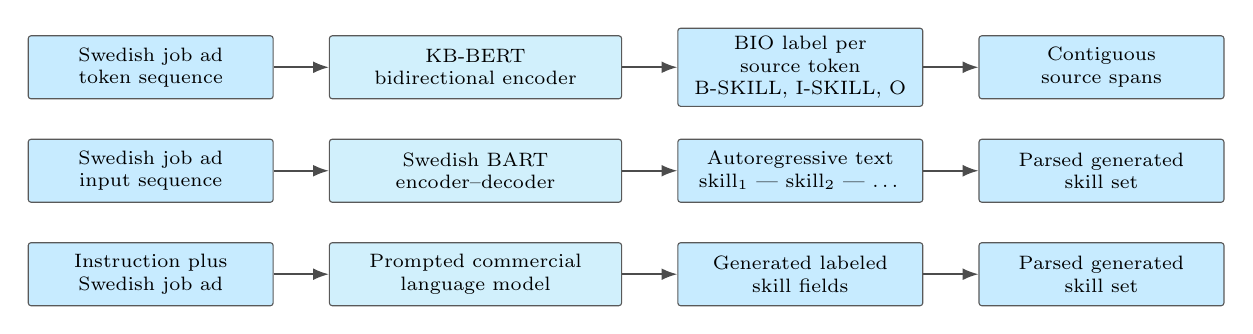
\begin{tikzpicture}[node distance=5mm and 7mm]
    \node[methodstage] (bertin) {Swedish job ad\\token sequence};
    \node[methodroute, right=of bertin] (bert) {KB-BERT\\bidirectional encoder};
    \node[methodstage, right=of bert] (biolabels) {BIO label per source token\\B-SKILL, I-SKILL, O};
    \node[methodstage, right=of biolabels] (bertout) {Contiguous\\source spans};

    \node[methodstage, below=5mm of bertin] (bartin) {Swedish job ad\\input sequence};
    \node[methodroute, right=of bartin] (bart) {Swedish BART\\encoder--decoder};
    \node[methodstage, right=of bart] (bartseq) {Autoregressive text\\skill$_1$ | skill$_2$ | \ldots};
    \node[methodstage, right=of bartseq] (bartout) {Parsed generated\\skill set};

    \node[methodstage, below=5mm of bartin] (llmin) {Instruction plus\\Swedish job ad};
    \node[methodroute, right=of llmin] (llm) {Prompted commercial\\language model};
    \node[methodstage, right=of llm] (llmseq) {Generated labeled\\skill fields};
    \node[methodstage, right=of llmseq] (llmout) {Parsed generated\\skill set};

    \foreach \a/\b in {bertin/bert,bert/biolabels,biolabels/bertout,
                         bartin/bart,bart/bartseq,bartseq/bartout,
                         llmin/llm,llm/llmseq,llmseq/llmout}
      \draw[methodarrow] (\a) -- (\b);
  \end{tikzpicture}
  \caption{\RVNOTE{hinh nay dung summarize 3 regimes tren dung ko?}\OURS{The three evaluated task formulations. KB-BERT is source-bound through BIO labels, whereas Swedish BART and the prompted systems generate text that must be parsed into skill sets.}}
  \label{fig:model-formulations}
\end{figure}

\section{Method}
\label{method}
\subsection{Task Formulation and Key Evaluation Approaches}
\label{keyapproaches}

%\RVNOTE{Subsection renamed from ``Key Approaches for Skill Extraction Evaluation'', now that it covers both the task definition and the evaluation measures. Running heads were also filled in: \emph{Language Models for Swedish Skill Extraction} and \emph{M. T. Nguyen et al.} And in the author list, ``Invesitgation'' is corrected to ``Investigation''.}

\subsubsection{Task Formulation}

Extraction locates or returns a mention such as ``continuous integration'', whereas normalization maps that mention to a canonical concept in a taxonomy such as ESCO. Recent production-oriented work likewise treats mention extraction and taxonomy linking as separate stages \citep{desanto2026skillens}. This study evaluates mention extraction that string normalization is an evaluation and post-processing operation but not an ESCO mapping. Accordingly, we formulate the task as mention extraction as follows: given a job ad and a target \OURSREV{view}{skill-label setting}, the system must identify skill mentions in the text without mapping them to an external taxonomy.

Let a job ad be represented by a token sequence $\mathbf{x}=(x_1,\ldots,x_n)$. For a target \OURSREV{view}{skill-label setting} $c$, the annotation used by the current implementation is a set of skill strings
\begin{equation*}
  \mathcal{G}^{*}_{c}(\mathbf{x})
  = \{g_1,\ldots,g_{K_c}\}.
\end{equation*}
Here, $c$ denotes one separately executed \OURSREV{view}{setting}: all skills, hard skills, soft skills, must-have skills, nice-to-have skills, or distinct skills. These \OURSREV{views}{setting} are not assumed to be mutually exclusive semantic classes. Each model run extracts a single entity type, \textsc{Skill}, for one fixed \OURSREV{view}{skill-label setting}. Duplicate surface forms are removed during canonicalization, so the evaluated object is a set rather than a multiset: repeated mentions of the same normalized skill are not counted repeatedly. The dataset stores skill strings rather than gold character offsets.

\subsubsection{Key Evaluation Approaches}

Two questions run through this study: how consistently do domain experts identify the same skills in the same job ad, and how closely does a model reproduce what those experts marked. Both are answered with the same set of measures, which are introduced here once and then used in Section~\ref{subsubsec:agreement} and Section~\ref{results}.

In both cases, the object being compared is a set of skill phrases. A system or a second annotator returns a set of phrases for one job ad. This set of phrases is compared with the set marked by the reference annotator. \emph{Precision} is the proportion of returned phrases that are correct, and answers the question of how far the output can be trusted. \emph{Recall} is the proportion of reference phrases that were returned, and answers the question of how much of what was there has been found. These two metrics can be traded against each other: a system that returns only the single most obvious skill has high precision and low recall, while a system that returns every noun phrase in the job ad has low precision and high recall. The $F_1$ score is the harmonic mean between precision and recall and is used throughout as a single summary that penalizes either extreme (see Equation \ref{eq:prf}). Formally, for a normalized predicted set $\mathcal{P}$ and a gold set $\mathcal{G}$, let $T$ be the number of one-to-one matched pairs under a specified matching rule; then

% [REV] Equation moved up from Section \ref{subsec:evaluation-method}, so that
% the agreement and the model-evaluation subsections can both refer to it here
% instead of each defining the measures again. It sits outside the shaded block
% only because framed cannot safely contain display maths.
\begin{equation}
  P=\frac{T}{|\mathcal{P}|},
  \qquad
  R=\frac{T}{|\mathcal{G}|},
  \qquad
  F_1=\frac{2PR}{P+R}.
  \label{eq:prf}
\end{equation}

Deciding which returned phrases count as correct requires a matching rule, and in this task the choice of rule matters more than the choice of measure. Under \emph{exact matching}, a returned phrase counts only if it is identical, character for character after normalization, to a reference phrase. \emph{Exact matching} is the conventional criterion in named entity recognition \citep{tjong2003conll}, and is strict in a way that suits skills poorly. For example, a system that returns \emph{C++} where the annotator wrote \emph{experience in C++} has identified the right competence, yet exact matching scores it as entirely wrong. Under \emph{boundary-relaxed containment matching}, this example pair is accepted because one complete normalized phrase contains the other. Containment therefore separates two kinds of error which exact matching conflates including failing to find a skill at all, and finding a skill but drawing its boundary in a different place \citep{andrade2023boundary}.

Both rules are reported throughout, and the difference between them is informative in its own right. \emph{Containment} is treated as the primary measure, because skill mentions in our Swedish data range from single words to expressions approaching a full sentence. Therefore, boundary variation is expected to be happened even between careful annotators working from the same guideline. Exact matching is reported alongside containment because containment in essence would hide how far the boundaries diverge and can credit a phrase that is broader than what was annotated. Additionally, two permissive rules including one based on token overlap and one on sentence-embedding similarity are also used but only as diagnostics and are defined in Section~\ref{subsec:evaluation-method}. 

\subsection{Manual Annotation}

\subsubsection{Data Collection}
This study started in the third quarter of 2025. At that time, only job ads of the first two quarter of 2025 were available in Arbetsförmedlingen. Thus, we decided to retrieve job ads of the two latest years starting from 2024 to the first two quarter of 2025 to make samples for this paper. Due to our team expertise and the contrasting skill profiles, we selected two domains including IT and journalism. However, each domain contains various job categories that cause a challenge in extracting consistent skill sets, such as graphic designers or data engineers in the IT field, and communication professionals and copy editors in the journalism field. Each job category owns different skill sets. Thus, we narrowed down the domains into two specific job categories: software developers (systemutvecklare in Swedish) and journalists (journalister or journalist/reporter in Swedish), that well-matched our team expertise and still reflected the contrasting skill profiles. After filtering out irrelevant job ads using the Swedish keywords, it was noticed that the gap in job ad numbers is considerable between these two job categories, namely 3150 job ads for software developers and 346 job ads for journalists. Due to the relatively small journalist dataset, we decided to use the entire dataset of journalists and randomly sample 10 percent of software developer job ads to obtain more comparable sample sizes across the two job categories.

%\begin{oursnewtext}
%The sampling unit was a complete job advertisement, identified by its source identifier. We retrieved advertisements posted from January 2024 through June 2025 and restricted the occupations to software developers (\emph{systemutvecklare}) and journalists (\emph{journalister} or \emph{journalist/reporter}). The source pool contained 3,150 software developer advertisements and 346 journalist advertisements. We retained all eligible journalist advertisements and drew a 10 percent random sample of the software developer pool, producing similarly sized corpora while preserving the two occupationally distinct writing styles.
%\end{oursnewtext}

The dataset was given in .csv format with a number of data fields among which we used three data fields: id, headline, and description. The column description was the primary data field that skills are extracted.


\subsubsection{Annotation Scheme}
\label{annotationscheme}
To design the annotation scheme, we skimmed through several job ads to obtain preliminary perspectives on how job ads in each job category were constructed and written. Afterwards, five labels were specified including \textit{hard skills}, \textit{soft skills}, \textit{distinct skills}, \textit{nice-to-have skills}, and \textit{must-have skills}. As a starting point for annotation, the labels were defined based on the general and commonly understood meanings of the relevant concepts (e.g., hard skills and soft skills), drawing on existing literature and the research team's domain knowledge. The definitions were intentionally kept simple and operational to facilitate consistent annotation.

\begin{itemize} 
\item \textit{Hard skills} refer to technical, tangible, and quantifiable abilities related to a field of work or study, typically acquired through training or education. \citep{lamri2023reconciling}
\item \textit{Soft skills} refer to personal, interpersonal, and intrapersonal abilities that are of necessity at workplace.\citep{lamri2023reconciling}
\item \textit{Distinct skills} refer to skills that are not typical to the job.
\item \textit{Nice-to-have skills} are identified if skills go with some keywords, such as meritorious, wish, bonus, a plus, good if you have, advantageous, or desirable (respectively to "meriterande", "önskvärt", "bonus", "plus", "bra om du har", "fördel", or "bra egenskap" in Swedish).
\item \textit{Must-have skills} are identified if skills go with some keywords, such as requirement, must, obligatory, required, important, or having experience on (respectively to "krav", "måste", "obligatoriskt", "krävs", "viktig", or "erfarenhet" in Swedish).
\end{itemize}

Furthermore, we proposed additional criteria to identify \textit{nice-to-have skills} and \textit{must-have skills} in case the annotators did not find the keywords mentioned above, namely including checking the positions of the skills in a job ad, checking frequency and emphasis, examining contextual language cues, and assessing the relation of skills with job title or job role (see Figure A1 in Appendix \ref{app:annotation} for the details of the annotation criteria). In case that the annotators could not specify whether a skill belongs to \textit{nice-to-have} or \textit{must-have}, they did not need to categorize it rather than only identifying it as \textit{hard skills}, \textit{soft skills}, or \textit{distinct skills}. We also defined \textit{nice-to-have skills} and \textit{must-have skills} as subsets of \textit{hard skills}, \textit{soft skills}, and \textit{distinct skills}. In other words, these labels indicate the importance or requirement level of a skill rather than representing additional skill categories. No new skills are introduced under the \textit{nice-to-have} or \textit{must-have} labels. Additionally, each skill should be kept as it is in the original text. This assignment was conducted using Microsoft Excel program. 

\subsubsection{Annotation Procedure}
The annotation process spanned nine months in total. Four annotators who speak Swedish and are experts in the respective fields engaged in the annotation assignment. Two were assigned for each job category and independently worked on this task following the given annotation design. Each annotator annotated a half of each dataset and additional about 10 percent overlapping data that we calculated agreement on. During manual annotation, 23 journalist job ads were found to be ineligible and one duplicated, and therefore were excluded without replacement, as no additional eligible journalist job ads were available. For software developers, ineligible job ads were replaced with randomly selected job ads from the remaining pool to maintain the target sample size. The detailed number of job ads for each researcher in each job is presented in Table \ref{tblJobAds}.
%\begin{oursnewtext} Đoạn này thay thế đoạn "The annotation process..." Annotation took nine months and involved four Swedish-speaking domain experts, two per occupation. Within each occupation, the two annotators received disjoint half-samples plus a fixed overlap sample used for agreement analysis: 32 software developer advertisements and 35 journalist advertisements. The overlap is therefore reported as a fixed audit sample rather than as exactly 10 percent of each final corpus. Of the 346 retrieved journalist advertisements, 23 were excluded as ineligible, leaving 323 annotated rows. Quality control then found two rows with the same identifier, headline, and description but different skill annotations. Source row 4 was retained and source row 313 was removed, leaving 322 unique journalist advertisements. No software developer identifier was duplicated. Table~\ref{tblJobAds} reports the resulting assignment. \end{oursnewtext}

\begin{table}[width=\textwidth,cols=6,pos=htbp]
\caption{Details of the annotation assignment.}\label{tblJobAds}
%\OLD{Original table terms: After human filter; 10 percent overlapping; System developers.}
%\OURS{Revised terms distinguish eligibility screening from duplicate removal and describe the fixed overlap sample.}
\begin{tabularx}{\textwidth}{Xccccc}
\toprule
Job category & Retrieved & \shortstack{After eligibility\\and duplicate checks} & \shortstack{Half of\\dataset} & \shortstack{Overlap\\sample} & \shortstack{Per annotator\\including overlap} \\
\midrule
Software developers & 315 & 315 & 158 & 32 & 190 \\
Journalists & 346 & 322 & 161 & 35 & 196\\
\bottomrule
\end{tabularx}
\end{table}

\subsubsection{Inter-Annotator Agreement}
\label{subsubsec:agreement}

Inter-annotator agreement was calculated on the overlapping independently-annotated samples to assess the consistency with which annotators identified and elaborated skills. This assessment was important because high model performance cannot compensate for inconsistencies in the underlying label definitions or the interpretation by domain experts \citep{artstein2008agreement,klie2024quality}. Following this assessment, disagreements were reviewed and discussed by the annotators to reach consensus. 

\begin{comment}
SkillSpan reports both token-level and exact-span agreement for offset-based
hard- and soft-skill annotations \citep{zhang2022skillspan}. The present data
store semicolon- or comma-separated mention strings rather than character
offsets, so token-level or exact-offset kappa cannot be reconstructed without
inventing annotation units.
\end{comment}

To calculate inter-annotator agreement, we used pairwise mention-set $F_1$. For every job ad, skill label, and job category, the two annotators' lists were normalized and deduplicated \NEW{using the same surface processing that is applied to model output in Section}~\ref{subsec:evaluation-method} \RVNOTE{em coi cho nay minh van refer den phan phia duoi, co on ko? Thuong ngta refer den phan phia tren???}. \OURSREV{}{Prediction-only filters were not applied to the inter-annotator reliability scoring.} One-to-one pairs were then assigned under the two matching rules defined in Section~\ref{keyapproaches} including normalized exact equality and boundary-relaxed containment. Counts were aggregated across the overlap sample and Equation~\ref{eq:prf} was applied to obtain micro $F_1$. %\NEW{, so the agreement figures and the model scores come from the same procedure and differ only in what is compared: two annotators here, a system against the reference annotator there}.

%\OLD{Exact-match} $F_1$ \OLD{measures agreement on the complete normalized phrase. Boundary-relaxed containment} $F_1$ \OLD{additionally recognizes cases in which one complete phrase contains the other.}
%\RVNOTE{Both sentences now repeat Section~\ref{keyapproaches}.}

Due to the linguistic characteristics of Swedish and two different job categories, the skills identified in this process varied considerably in span length (see the example annotations in Figure \ref{FIG:Label_Journal} and \ref{FIG:Label_IT}). Skills were expressed not only as single words but also as multi-word phrases and, in some cases, longer expressions approaching a full sentence. Therefore, we primarily relied on the boundary-relaxed containment scores to assess inter-annotator agreement, as this measure is more appropriate for capturing semantically consistent annotations that may differ slightly in span boundaries \citep{malandri2025skillmo}. Additionally, the difference between the exact-match and boundary-relaxed containment scores is interpreted as reflecting variation in span boundaries and phrase length rather than disagreement in the skill identification. The low exact scores are explained by a small number of mentions available and the strict criteria of considering ``matching'', while the boundary-relaxed containment is calculated based on the relaxed criteria. The agreement scores are shown in Table \ref{tab:inter-annotator-agreement}. The scores in the boundary-relaxed containment are between 0.7 and 1, indicating substantial consistency between the annotators. %once differences in span boundaries are set aside.  

\begin{figure}
	\centering
		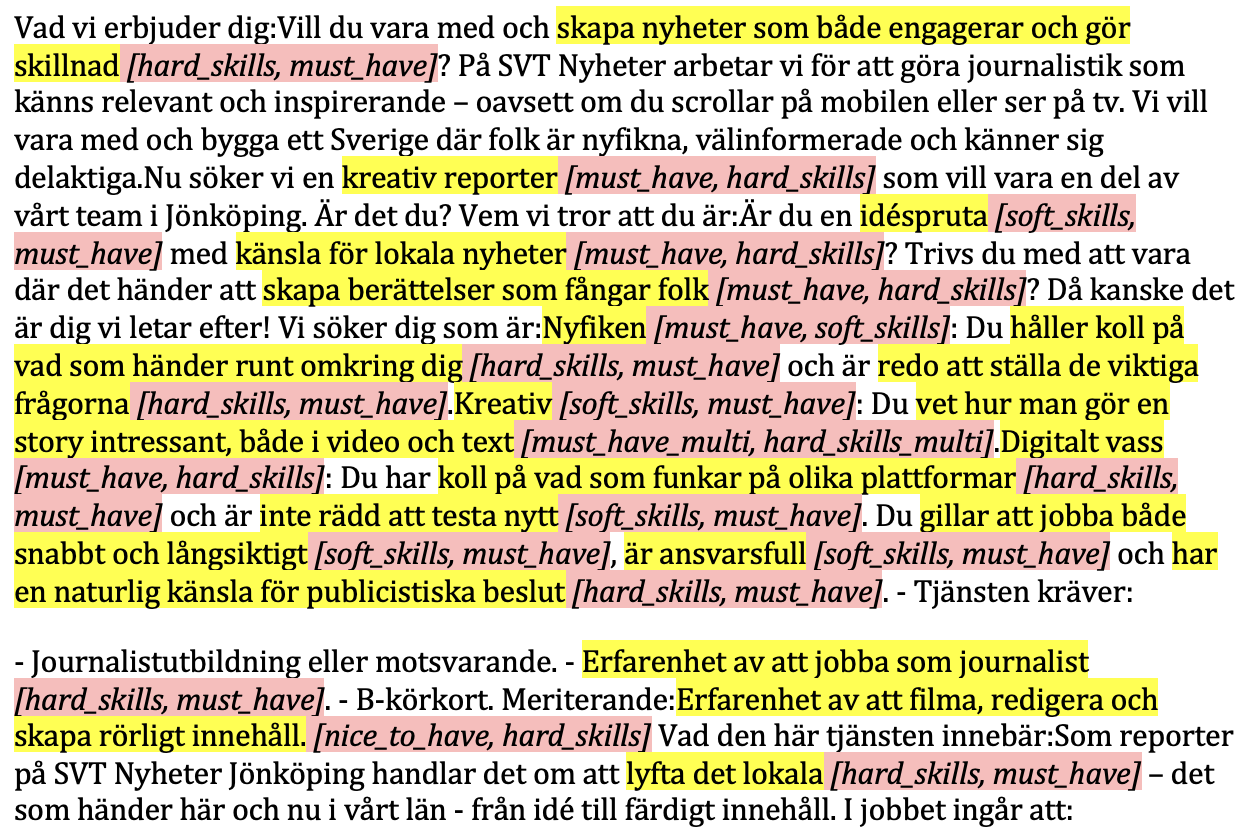
\includegraphics[scale=.55]{figs/Label_Journal.png}
	\caption{Example annotations of a journalist job ad}
	\label{FIG:Label_Journal}
\end{figure}

\begin{figure}
	\centering
		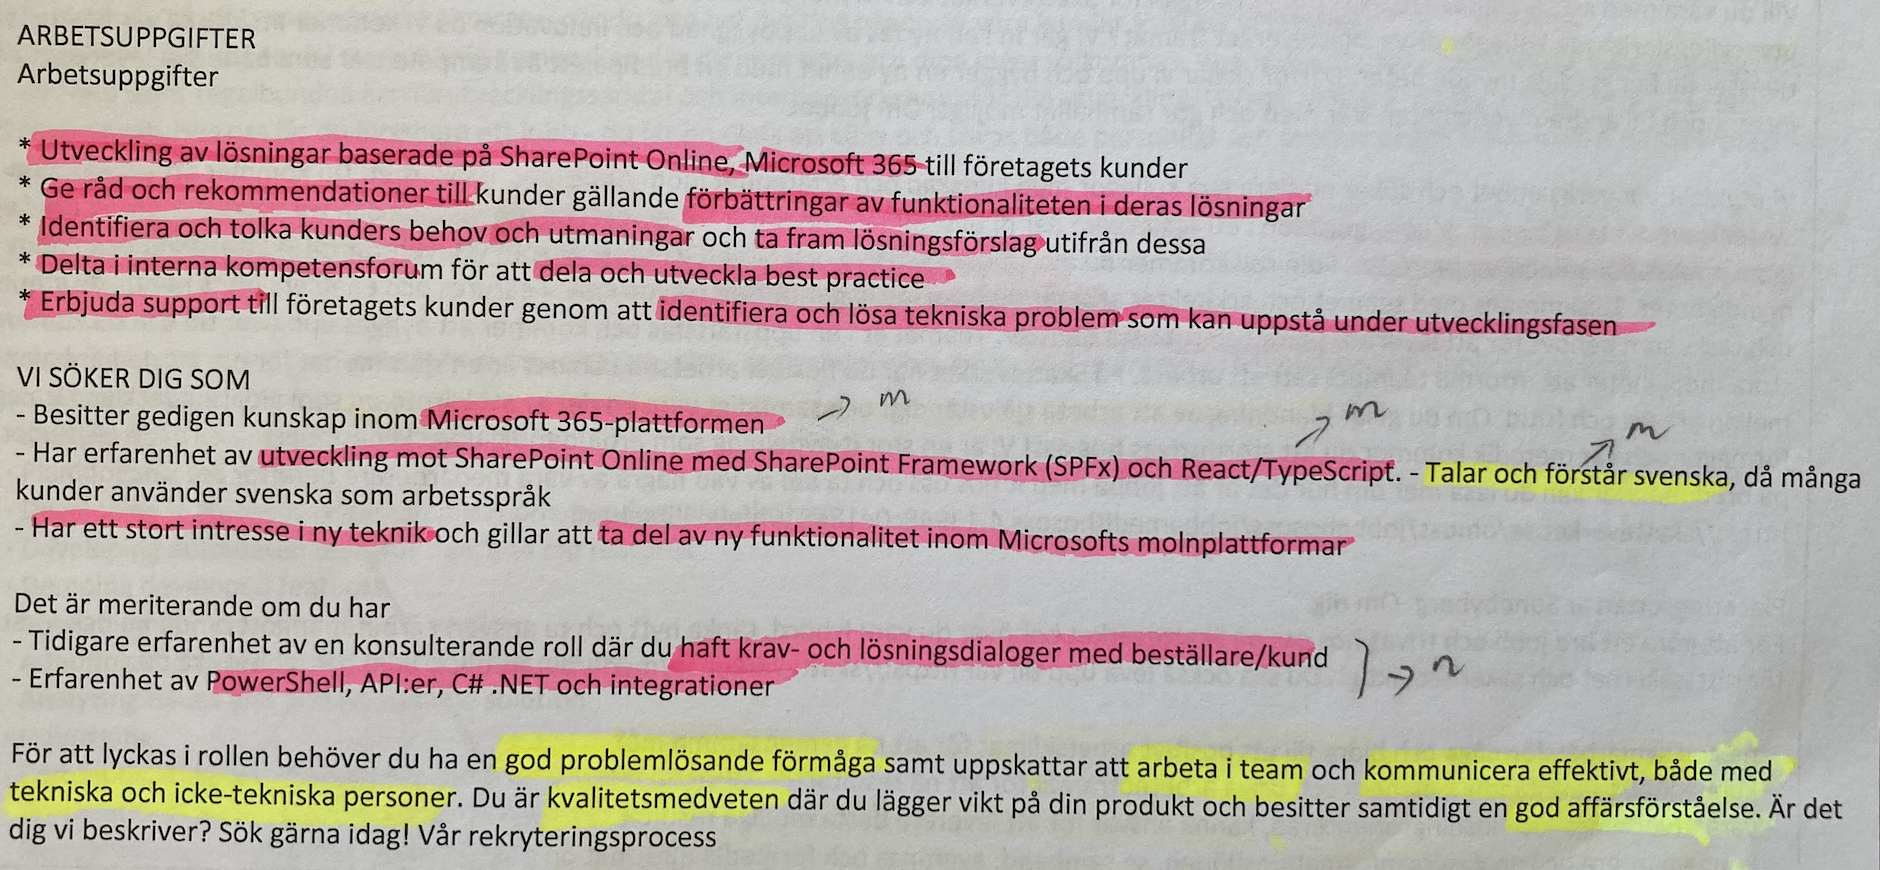
\includegraphics[scale=.35]{figs/Label_IT.png}
	\caption{Example annotations of a software developer job ad}
	\label{FIG:Label_IT}
\end{figure}

\begin{table}[H]
  \centering
  \small
  \caption{Pairwise inter-annotator agreement on independently annotated
  advertisements. Values are micro $F_1$ over one-to-one mention matches.}
  \label{tab:inter-annotator-agreement}
  \begin{tabular}{llrrr}
    \toprule
    Job categories & Skill label & Records & Exact & \shortstack{Boundary-relaxed\\containment} \\
    \midrule
    Software developers & Hard skills & 32 & \OURSREV{0.698}{0.692} & \OURSREV{0.893}{0.882} \\
    Software developers & Soft skills & 32 & \OURSREV{0.673}{0.676} & \OURSREV{0.888}{0.889} \\
    Software developers & Distinct skills & 32 & 0.667 & 1.000 \\
    Software developers & Must-have skills & 32 & \OURSREV{0.662}{0.652} & \OURSREV{0.923}{0.914} \\
    Software developers & Nice-to-have skills & 32 & \OURSREV{0.705}{0.701} & \OURSREV{0.949}{0.948} \\
    \midrule
    Journalists & Hard skills & 35 & \OURSREV{0.562}{0.489} & \OURSREV{0.831}{0.792} \\
    Journalists & Soft skills & 35 & \OURSREV{0.762}{0.763} & \OURSREV{0.846}{0.844} \\
    Journalists & Distinct skills & 35 & \OURSREV{0.457}{0.407} & \OURSREV{0.714}{0.712} \\
    Journalists & Must-have skills & 35 & \OURSREV{0.665}{0.620} & \OURSREV{0.884}{0.856} \\
    Journalists & Nice-to-have skills & 35 & 0.791 & 0.977 \\
    \bottomrule
  \end{tabular}
\end{table}

%The overlap annotations were retained for reliability analysis, while the modeling dataset contains one consolidated annotation per identifier. The available annotation records do not preserve a complete adjudication log. This absence limits claims about how disagreements were resolved and is reported as a data-documentation limitation rather than replaced by an inferred procedure.


\subsection{Transformer-based Models}

While section~\ref{background} described what encoder-only and encoder--decoder transformers are and how each represents an extraction task, this subsequent section turns to the choices this study actually made including which Swedish  checkpoints were used and why, and how the annotation described above was turned into training data for each of the two formulations \RVNOTE{what are the two formulations?}.

\subsubsection{Why BERT and BART are Appropriate Reference Models}

In this study, BERT and BART are selected as canonical Swedish-language reference architectures, not as state-of-the-art representatives at present. They provide a clear correspondence between two established formulations: encoder-only BIO classification and encoder--decoder conditional generation. The National Library of Sweden provides checkpoints for both families. KB-BERT was developed to provide Swedish contextual representations \citep{malmsten2020swedishbert}, and a Swedish BART checkpoint is available for sequence-to-sequence modeling \citep{kblab2021bart}. Language matching reduces the obvious confound of comparing a Swedish checkpoint against an English-only checkpoint.

However, language matching does not isolate architecture. The selected checkpoints can still differ in pretraining data, objectives, tokenizers, parameterization, and optimization history; the task systems additionally differ in supervision alignment, output space, post-processing, and decoding. They should therefore be called \emph{language-matched reference architectures} but not controlled architectural replicates. Any conclusion must be stated at the configuration level, for example, ``KB-BERT with BIO labeling outperformed Swedish BART with serialized generation under the evaluated settings'', rather than generalized to all encoder-only and encoder--decoder models.%\RVNOTE{This caveat is made a third time in Section~\ref{subsec:limitations} and once more in the Discussion. Proposed: keep it here, where the choice of checkpoints is being justified, and shorten the other two to a cross-reference.}

\subsubsection{BERT Operation in Skill Extraction}

In Section~\ref{keyapproaches}, the annotation for one job ad was defined as a set of skill strings but not as marked positions in the text. However, an encoder-only model predicts a label for every token, so the strings have to be located in the job ad before training can begin. This step and the supervision it produces is what distinguishes this formulation \RVNOTE{which formulation? } from the generative one described next \RVNOTE{which one is next?}.

For the BERT formulation, training spans are derived by matching each $g_k$ back to the source text. If $\operatorname{match}(g_k,\mathbf{x})$
returns its case-insensitive, contiguous surface occurrences, the weakly aligned span set is
\begin{equation*}
  \mathcal{A}_{c}(\mathbf{x})
  = \bigcup_{g\in\mathcal{G}^{*}_{c}(\mathbf{x})}
    \operatorname{match}(g,\mathbf{x}).
\end{equation*}
Only strings found in the job ad contribute BIO labels. Consequently, the supervised token-labeling data are weaker than manually annotated offset spans: an unmatched paraphrase supplies no token-level supervision, and ambiguous repeated surface forms are all matched.

BIO encoding marks the beginning, continuation, and exterior of a contiguous span with \texttt{B-SKILL}, \texttt{I-SKILL}, and \texttt{O}, respectively \citep{ramshaw1995chunking}. This directly represents flat, contiguous mentions, but not nested, overlapping, or discontinuous mentions as independent entities. This is consequential for skills, which may be syntactically complex or context dependent \citep{nguyen2024rethinking}. In the current alignment code, when two candidate spans overlap a token, the longer span determines the label. The BERT hypothesis space is therefore structurally restricted in a way that the generative systems are not.

\subsubsection{BART Operation in Skill Extraction}

Whereas the encoder-only system labels tokens that are already present in the job ad, the encoder--decoder system is trained to write the answer out. \OURSREV{For one job ad and one skill label, the annotated skill set is serialized into a single target string in which the individual skills are separated by a vertical bar.}{Each gold skill is assigned to every chunk containing its normalized contiguous token sequence, or to the chunk with greatest token-set overlap if none contains it, and each chunk target is serialized with vertical-bar delimiters.} BART receives \OURSREV{the job ad description}{the stripped headline and description joined by a newline} as input and learns to reproduce the string one token at a time, by minimizing the conditional generation loss in Equation~\ref{eq:bart-loss}. During training, \NEW{BART} \OLD{the decoder} is supplied with the correct preceding tokens at each step, a standard procedure known as teacher forcing. At test time, \NEW{BART} \OLD{the decoder} generates without that assistance, using beam search, which keeps several candidate continuations under consideration before committing to one.

This formulation \RVNOTE{which? where?} carries one clear advantage over BIO tagging and one clear cost. \OURSREV{The advantage is that the target is the advertisement-level skill list rather than a set of positions in the text, so no surface-alignment step is required.}{The advantage is that BART generates a skill list rather than BIO token positions, while source-to-chunk target alignment is used during training.} An annotated skill that appears in the job ad only as a paraphrase, or as a discontinuous expression that flat BIO tagging cannot represent, still contributes to training instead of being skipped. The cost is that the output space is unconstrained. The model must learn what to extract, how to render it, and how to delimit it, all from the same small training signal, and nothing in the architecture prevents it from returning a phrase that does not occur in the job ad at all. Parsing the generated string back into a set of skills is consequently also the point at which delimiter errors, duplicated items, and unsupported strings enter the results. This asymmetry between a source-bound and a freely generating output space is used in Section~\ref{discussions} to interpret the difference between the two supervised systems.


\subsection{Large Language Model-Based Methodology}
\label{LLMMethod}
% include prompt creation by the selected tool
To compare with the transformer-based models, we selected three of the latest and most widely used LLMs available at the time of the study including GPT-5, Gemini-3.5-flash, and Claude-Sonnet-4-6 (See Table \ref{tblparadigms} for the detailed comparison between the transformer-based models and LLMs). All three models support multiple languages, including Swedish, and are accessible through APIs. Namely, we set 5 calls per job ad, one independent request per skill label and single sample each. In total, we performed 3185 calls for each LLM in both job categories. Moreover, GPT was set with four retries as maximum and an exponential backoff strategy, with waiting times capped at 30 seconds. The resulting retry delays were 1, 2, 4, and 8 seconds. Retries were performed only when the error message contained one of the following indicators: 429, rate, timeout, temporary, overload, 500, 502, 503, or 504. Meanwhile, Gemini API calls were implemented with a maximum of five retries and an initial delay of 2.0 s, following an exponential backoff schedule of 2, 4, 8, and 16 seconds. Retries were triggered for API errors with codes 429 or 503, and for connection exceptions. In addition, a one-second delay was set between job ads. For Claude, no retry mechanism was implemented. When encountering a RateLimitError, the process paused for 60 s before continuing. All these API runs were performed between around the end of March and May 2026. To maximize the quality and consistency of the generated results, we developed separate prompts for each label–LLM combination. Thus, a total of fifteen prompts were created, corresponding to the five labels and three LLMs.  

%\RVNOTE{Section~2.3 states that reproducible evaluation requires ``the exact model identifier or snapshot, access date, full prompt, generation settings, parsing rules, retry policy, and number of repeated calls''. None of these is currently given here, so the manuscript sets a standard it does not meet. Please add a short paragraph or a table with the exact API model strings, the access dates, temperature and other decoding settings, the retry policy, and the number of calls per advertisement. Note also that \emph{Gemini-3.5-flash} is not a released identifier and \emph{Claude-Sonnet-4-6} is nonstandard formatting; both need to be replaced by the strings actually sent to the API.} 


\subsubsection{Prompt Generation}
\label{subsubsec:prompt-generation}

The initial prompts were generated using Metagente - an LLM-based multi-agent system for automated prompt optimization \citep{nguyen2026automated}. The prompt generation followed the Metagente pattern of iterative multi-agent prompt optimization \citep{nguyen2025metagente}. A target-specific initial prompt instructed a summarizer agent to return only Swedish skill phrases, preserve wording from the job ads, remove duplicates, and separate items with semicolons. During prompt development, a teacher agent received the current prompt, a training advertisement, the GPT-generated skill list by the summarizer agent, the corresponding reference list, and an automatically calculated performance score. When the score did not meet the acceptance threshold, the teacher agent proposed a minimal revision to the prompt. Candidate prompts associated with qualified examples were then aggregated by a prompt-combination agent into one final prompt for each skill label. The optional extractor agent was bypassed, so the complete job ad was passed directly to the summarizer agent, which ran at temperature zero. The final optimized prompt contained no in-context demonstrations, so evaluation used a zero-shot \emph{prompt format}. Prompt optimization nevertheless used the labeled development examples. The LLM regime is therefore parameter-free at inference but not label-free during system development. % \OLD{The distinction is retained in the comparison and discussion.}\RVNOTE{Proposed cut: the sentence announces that a distinction will be respected later rather than stating anything about the method.}

Following the automated prompt generation process, we conducted manual testing of the resulting prompts on a small sample for each skill label and LLM. These tests revealed that some relevant skills were not consistently extracted by the initial prompts. We therefore iteratively revised the prompts to improve their coverage of relevant skills. The final prompts are found in \colorbox{yellow}{Appendix}~\ref{app:prompts}.


\begin{table}[width=.9\linewidth,cols=5,pos=h]
\caption{Conceptual comparison of the evaluated modeling paradigms.}\label{tblparadigms}
\begin{tabular*}{\tblwidth}{@{}p{1.6cm}p{2.7cm}p{2cm}p{2.5cm}p{4cm} LLLLL@{} }
\toprule
System & Architecture & Adaptation & Study output & Principal constraint or risk\\
\midrule
KB-BERT & Encoder only & Full supervised fine-tuning & BIO spans converted to a skill set & Contiguous source spans; weak surface alignment; no nested or overlapping output \\
    Swedish BART & Encoder--decoder & Full supervised fine-tuning & Serialized sequence parsed as a skill set & Unconstrained generation, delimiter errors, paraphrases, and unsupported output \\
    Prompted LLMs & Provider-dependent generative systems & Prompting with fixed parameters & Generated fields parsed as skill sets & Prompt and version sensitivity, format failures, and unsupported output \\
\bottomrule
\end{tabular*}
\end{table}

% \subsection{Fine-Tuning}
% \subsubsection{Reflection on Validation-Based Framework Selection}
% Pretraining supplies general language representations; fine-tuning adapts a pretrained model to labeled task data by updating its parameters \citep{howard2018ulmfit,devlin2019bert}. In this study, both supervised systems use full fine-tuning. BERT learns the token objective in Equation~\ref{eq:bert-loss}, whereas BART learns the conditional generation objective in Equation~\ref{eq:bart-loss}. Optuna is not itself a fine-tuning method. It is the framework used to select hyperparameters for those fine-tuning procedures \citep{akiba2019optuna}.

% Let $\lambda\in\Lambda$ denote a hyperparameter configuration and let $\theta$ denote trainable model parameters. Validation-based selection can be written as the nested problem
% \begin{equation}
%   \theta^{*}(\lambda)
%   = \arg\min_{\theta}\mathcal{L}_{\mathrm{train}}(\theta;\lambda),
%   \qquad
%   \lambda^{*}
%   = \arg\max_{\lambda\in\Lambda}
%     F_{1,\mathrm{val}}\!\left(\theta^{*}(\lambda)\right).
%   \label{eq:hpo}
% \end{equation}
% The selected configuration is then evaluated on held-out test data. This separation matters because repeatedly using test performance for model selection yields optimistic estimates \citep{cawley2010selection}.

% Fine-tuning can be sensitive to data order, head initialization, and random seed, particularly in small datasets \citep{dodge2020finetuning}. A defensible experiment must therefore report the search space, trial count, validation objective, sampler and its seed, pruning or stopping behavior, final training rule, and variation across repeated training seeds. Equal trial counts also do not necessarily imply equal compute budgets when architectures and decoding costs differ.

% The study additionally reports no-task-training controls. Their interpretation requires care. A pretrained BART checkpoint already has a trained generative decoder, although it has not learned the study's skill serialization. By contrast, loading pretrained BERT into a three-label token-classification model creates a newly initialized classification head. The no-fine-tuning BERT result is therefore an initialization control with an untrained task head, not a meaningful zero-shot BERT extractor. It should not be described as BERT's general skill-extraction ability ``before fine-tuning.''
\subsection{Fine-Tuning}
\label{subsec:finetuning-method}

In Section \ref{background}, fine-tuning was introduced as the regime in which the model's own parameters are changed by training on annotated examples. This regime applied to this study is explained in this section. 

Supervised fine-tuning continues optimization on annotated task data so that model parameters support a specific prediction objective \citep{howard2018ulmfit,devlin2019bert}. Full fine-tuning updates the pretrained parameters together with the task-specific output components. In this study, BERT configuration minimizes Equation~\ref{eq:bert-loss}, while BART configuration minimizes Equation~\ref{eq:bart-loss}.

%gioi thieu ve cac hyper parameter
A complete training run includes several steps: task-data construction, tokenization or target serialization, model initialization from a pretrained checkpoint, mini-batch optimization, hyperparameter selection based on validation performance, model reinitialization with the selected configuration, and one final test evaluation. These settings interact strongly when the training set is small. The range of values searched and the rule used to choose among them are therefore part of the experimental method rather than implementation detail, and both are presented in the subsequent sections. %\OLD{Additionally, the primary hyperparameters control different aspects of the training: the learning rate controls update magnitude; batch size and gradient accumulation determine the effective batch; epoch count controls exposure to the training data; weight decay regularizes parameter magnitude; warm-up stabilizes early updates; label smoothing changes the encoder--decoder target distribution; and beam width controls validation-time generation.}\RVNOTE{Proposed cut: this glossary names the same seven hyperparameters that Table~\ref{tab:hpo-space} lists with their search ranges, so the reader meets them twice. The table is the more informative of the two.} These choices can interact strongly on small datasets, so \colorbox{yellow}{cau nay ko ro nghia? the search space and selection rule form part of the experimental method.}\NEW{[proposed rewording: ``'']}

In this study, separate transformer-based models were trained for each combination of model family, job category, and skill label. The two job category settings and one synthetic setting include software developers, journalists, and the merged corpus. The five annotated skill labels and one synthetic label include hard skills, soft skills, distinct skills, must-have skills, nice-to-have skills, and all skills. The factorial design produced 18 fine-tuned configurations per model family and 36 fine-tuned configurations in total.

For each configuration, records were partitioned by identifier into 40\% training, 10\% validation, and 50\% test data using seed 13. The implementation stratified the split by quantile bins derived from \OURSREV{must-have and nice-to-have list lengths}{input-word count, target-item count, and target-word count, with all-skills also using five component-label counts and merged also using occupation membership}. Hyperparameters were selected only on the validation partition, and the selected model was evaluated once on the test partition. The same canonical test identifiers were used for the prompted models and the task-unadapted controls within every job category--skill configuration.

% Quality control identified two journalism source rows with the same identifier,
% headline, and description but different skill annotations. In the frozen source
% file, row 4 was retained and row 313 was removed. Split assignments for every
% other record were preserved. Because the duplicate rows occupied different
% partitions across the stratified skill-view splits, the 12 BERT or BART
% configurations in which the removed row had affected training or validation
% were fine-tuned again. Configurations affected only at test time were corrected
% by retaining or filtering the appropriate row and recomputing the metrics;
% task-unadapted baselines and GPT, Claude, and Gemini were not re-executed, and
% their existing predictions were identifier-aligned and rescored. The final
% audit verified 12 of 12 reruns, exact identifier and gold-label alignment for
% all 72 BERT/BART outputs, and test alignment for all 54 prompted-model outputs.

\subsubsection{BERT Fine-Tuning Procedure}

BERT training proceeded in six steps. First, the Swedish BERT checkpoint was loaded with a newly initialized three-label token-classification head. Second, each \OURSREV{annotated skill string was located in the description}{skill string was located in the shared headline--description input} by a case-insensitive regular expression that permitted whitespace variation and normalized dash characters. Third, advertisements with no target skills or no surface-alignable target spans were excluded from token-level training. Fourth, \OURSREV{descriptions}{the shared inputs} were tokenized into windows of at most 512 subwords with a stride of 128; subwords overlapping the longest applicable gold span received \emph{Beginning} or \emph{Inside} labels. Fifth, \OURSREV{cross-entropy}{weighted cross-entropy} loss was minimized for the selected epoch count and optimization settings\OURSREV{}{ across all 18 BERT configurations}. Sixth, test-time predictions from overlapping windows were mapped to source offsets, overlapping predicted spans were merged, and isolated Inside labels were decoded as new spans. Training\OURSREV{ and validation}{, validation, and test} used \OURSREV{the description field; final test inference combined headline and description, as implemented in the executed notebooks}{the stripped headline and description joined by a newline}.

The training procedure used full parameter updating and no conditional random field. Skipping unmatched annotations prevented incorrect token labels, but the same decision changed the effective training sample and removed negative-only job ads from supervised learning (see Table \ref{tab:bert-effective-training} for the details).%\RVNOTE{The number of retained and skipped records per skill label is not yet anywhere in the manuscript, and a reviewer will ask for it, because skipping unmatched annotations changes the effective training set.}
% advertisements from supervised learning. The number of retained and skipped
% records should therefore be reported for every skill view.

\begin{table*}[width=\textwidth,pos=htbp]
  \centering
  \scriptsize
  \setlength{\tabcolsep}{4pt}
  \caption{Effective BERT training records after surface alignment on the corrected seed-13 split. ``No-span skipped'' counts records with a nonempty target list for which no target string aligned to the source. ``Other excluded'' covers an empty input or target removed by the notebook preprocessing.}
  \label{tab:bert-effective-training}
  \begin{tabular}{llrrrr}
    \toprule
    Job category & Skill label & Split train & Retained & No-span skipped & Other excluded \\
    \midrule
    Software developers & All skills & 126 & 126 & 0 & 0 \\
    Software developers & Hard skills & 125 & 125 & 0 & 0 \\
    Software developers & Soft skills & \OURSREV{123}{122} & \OURSREV{123}{122} & 0 & 0 \\
    Software developers & Distinct skills & 33 & 33 & 0 & 0 \\
    Software developers & Must-have skills & \OURSREV{113}{114} & \OURSREV{113}{114} & 0 & 0 \\
    Software developers & Nice-to-have skills & \OURSREV{67}{66} & \OURSREV{67}{66} & 0 & 0 \\
    \midrule
    Journalists & All skills & \OURSREV{66}{129} & \OURSREV{66}{129} & 0 & 0 \\
    Journalists & Hard skills & \OURSREV{129}{128} & \OURSREV{129}{128} & 0 & 0 \\
    Journalists & Soft skills & 113 & 113 & 0 & 0 \\
    Journalists & Distinct skills & \OURSREV{78}{79} & \OURSREV{77}{78} & 1 & 0 \\
    Journalists & Must-have skills & 128 & 128 & 0 & 0 \\
    Journalists & Nice-to-have skills & \OURSREV{70}{71} & \OURSREV{70}{71} & 0 & 0 \\
    \midrule
    Merged & All skills & \OURSREV{193}{255} & \OURSREV{192}{255} & 0 & \OURSREV{1}{0} \\
    Merged & Hard skills & \OURSREV{253}{254} & \OURSREV{253}{254} & 0 & 0 \\
    Merged & Soft skills & 236 & 236 & 0 & 0 \\
    Merged & Distinct skills & 112 & 111 & 1 & 0 \\
    Merged & Must-have skills & \OURSREV{244}{243} & \OURSREV{244}{243} & 0 & 0 \\
    Merged & Nice-to-have skills & \OURSREV{138}{137} & 137 & \OURSREV{1}{0} & 0 \\
    \bottomrule
  \end{tabular}
\end{table*}

\subsubsection{BART Fine-Tuning Procedure}

BART training began from the Swedish pretrained checkpoint. The input was the \OURSREV{job ad description}{stripped headline and description joined by a newline}, and the target was a vertical-bar separated list of skills for one \OURSREV{}{skill-label setting}. \RVNOTE{view?} Job ads with empty target lists were excluded from training. Source texts longer than 1,000 tokens were divided into overlapping chunks with 160-token overlap. \OURSREV{Each chunk was paired with the complete advertisement-level target list.}{Every annotated skill was paired with every chunk containing its normalized contiguous token sequence, or if no such chunk existed, with the chunk exhibiting the greatest token-set overlap.} Inputs and targets were truncated to 1,024 and \OURSREV{96}{512} tokens, respectively.

Teacher-forced conditional generation loss was minimized with the trial-specific learning rate, batch size, gradient accumulation, epoch count, weight decay, label smoothing, and warm-up ratio. \OURSREV{Training inputs used the description. Validation and final test generation combined headline and description.}{Training, validation, and final test inputs all utilized the same stripped headline and description joined by a newline.} Validation used beam width two. Final generation used beam width six, at most \OURSREV{96}{512} new tokens, and a no-repeat $n$-gram size of three. Generated lists from all chunks were merged\OURSREV{ and normalized duplicates were removed}{, and only exact normalized duplicates were removed while distinct nested phrases were preserved}. \OURSREV{Pairing every long-text chunk with the complete advertisement-level target can expose a chunk to target skills absent from that chunk. The resulting weak chunk-level supervision is seen as a limitation.}{Deterministic token-overlap fallback assignments for skills not found in any chunk may still provide weak chunk-level supervision.}

\subsubsection{Validation-Based Hyperparameter Selection}
\label{subsubsec:hpo-method}

%toi uu va gioi thieu framework dung thuat toan do
Hyperparameter optimization is a separate layer around fine-tuning. To optimize the hyperparameter selection, we used the framework Optuna. Optuna provides the search framework used to propose and evaluate configurations rather than a fine-tuning objective \citep{akiba2019optuna}. 

Let $\lambda\in\Lambda$ denote learning rate, batch size, epoch count, regularization, and other training or decoding choices. Validation-based selection can be
written as
\begin{equation}
  \theta^{*}(\lambda)
  = \arg\min_{\theta}\mathcal{L}_{\mathrm{train}}(\theta;\lambda),
  \qquad
  \lambda^{*}
  = \arg\max_{\lambda\in\Lambda}
    F_{1,\mathrm{validation}}
      \!\left(\theta^{*}(\lambda)\right).
  \label{eq:hpo}
\end{equation}
 The held-out test set is consulted only after
$\lambda^{*}$ has been selected, because repeated test-guided selection can
produce optimistic performance estimates \citep{cawley2010selection}. %\colorbox{yellow}{den day xem co dung logic ko?}\RVNOTE{Yes. This is the standard protocol and it is correctly described: the configuration is chosen on the validation partition only, and the test partition is consulted once, after that configuration is fixed. The shared split and seed that make the 36 configurations comparable are already stated in Section~\ref{subsec:finetuning-method}, so nothing needs adding.}

Optuna executed 20 trials independently for every model--job category--skill configuration. Every trial reloaded the pretrained checkpoint, trained a new model on the training partition, generated or decoded predictions on the validation partition, and returned \OURSREV{macro boundary-relaxed containment $F_1$}{exact normalized macro $F_1$}. The optimization objective therefore corresponds to \OURSREV{exact matches plus containment matches}{exact matches}; \OURSREV{lexical and semantic relaxation}{containment, lexical, and semantic matching} did not determine the selected hyperparameters.

\begin{table}[H]
  \centering
  \small
  \setlength{\tabcolsep}{4pt}
  \caption{Hyperparameter search spaces implemented for the supervised
  reference configurations.}
  \label{tab:hpo-space}
  \begin{tabular}{lll}
    \toprule
    Hyperparameter & Encoder-only search space & Encoder--decoder search space \\
    \midrule
    Learning rate & Log-uniform $[10^{-5},8\times10^{-5}]$ & Log-uniform $[10^{-5},8\times10^{-5}]$ \\
    Training batch size & $\{4,8\}$ & $\{1,2,4\}$ \\
    Gradient accumulation & $\{1,2,4\}$ & $\{1,2,4\}$ \\
    Epochs & Integer $[2,5]$ & Integer $[2,6]$ \\
    Weight decay & Continuous $[0,0.05]$ & Continuous $[0,0.05]$ \\
    Label smoothing & Not searched & Continuous $[0,0.15]$ \\
    Warm-up ratio & Not searched & Continuous $[0,0.10]$ \\
    Validation beam width & Not applicable & 2 \\
    \bottomrule
  \end{tabular}
\end{table}

After 20 trials, the configuration with the highest validation objective was selected. A fresh copy of the pretrained model was then initialized and trained on the training partition using the selected parameters. The validation set was not merged into final training, and the implementation did not use early stopping or checkpoint selection within the final run. Test evaluation used the resulting final epoch.

Both the training seed and the data seed were fixed at 13, and \OURSREV{the sampler and pruner were left at the Optuna defaults}{the sampler was set to TPESampler(seed=13) while the pruner remained at the Optuna defaults}. Equal trial counts across the two model families should not be read as equal compute budgets because encoder--decoder generation is more expensive than encoder-only decoding. The consequences of running a single seed are taken up in Section~\ref{subsec:limitations}.


%\OLD{The code sets both training and data seed to 13 and executes only \texttt{SEEDS = [13]}. Comments referring to three seeds are stale and do not describe the executed experiment. Optuna's sampler, sampler seed, and pruner were not explicitly configured in the scripts, so the installed Optuna defaults governed trial proposals and pruning behavior. A reproducible report must record the Optuna and dependency versions or explicitly instantiate a seeded sampler in a future rerun. Equal trial counts should not be interpreted as equal compute budgets, because encoder--decoder generation is more expensive than encoder-only decoding.} \RVNOTE{Proposed cut, replaced by the shorter paragraph above. This one is written as a note to ourselves about the code (``comments referring to three seeds are stale'', ``a reproducible report must record the Optuna and dependency versions''), which is not a statement about the study. The single seed is already reported as a limitation.}

\subsection{Model Evaluation}
\label{subsec:evaluation-method}

Section~\ref{keyapproaches} introduced the metrics precision, recall, $F_1$, exact matching, and boundary-relaxed containment matching, which are employed for the model evaluation. Equation~\ref{eq:prf} is applied to the counts described below. This part specifies only what is particular to evaluating model output rather than comparing two annotators, namely how predictions and gold lists are normalized before they are compared, the order in which candidate matches are assigned, and how per-advertisement scores are aggregated.

\begin{comment}
\OLD{Exact span evaluation traditionally requires a predicted entity to reproduce the complete gold boundary} \citep{tjong2003conll} \OLD{. Exact matching is transparent and conservative, but exact matching can treat ``C++'' and ``experience in C++'' as entirely different even when both outputs identify the same central technical competence. Boundary-relaxed evaluation can therefore be reported as a complementary view, provided that the matching rule is explicit and exact results remain visible} \citep{andrade2023boundary} \OLD{.}

\OLD{Exact-match} $F_1$ \OLD{counts only normalized string equality. The present study also reports} \emph{boundary-relaxed containment $F_1$}\OLD{, which first assigns exact matches and then accepts a remaining prediction--gold pair when either normalized string contains the other.}
\RVNOTE{These two paragraphs now repeat Section~\ref{keyapproaches}, including
the same ``C++'' example, so they are proposed for deletion. The citations they
carry, \citet{tjong2003conll} and \citet{andrade2023boundary}, have been moved
up to Section~\ref{keyapproaches} so that nothing is lost.}

%The term ``partial match'' is avoided because partial matching may refer to any token overlap, boundary overlap, or fractional credit in other studies. Containment is the exact operation used by the implementation.?? maybe remove?}
\end{comment}

Two broader diagnostic levels are also available. Lexically relaxed matching
uses the larger of multiset token-overlap $F_1$ and longest-common-subsequence
$F_1$; the latter is related to ROUGE-L \citep{lin2004rouge}. Semantically
relaxed matching compares Swedish sentence embeddings with cosine similarity,
following the general sentence-embedding principle introduced by Sentence-BERT
\citep{reimers2019sentencebert}. Broader matching can reveal morphology or
paraphrase sensitivity, but broader matching can also credit a phrase that is
not an exact source mention. Exact and containment scores are therefore the
main results, while lexical and semantic scores are supporting diagnostics.

\subsubsection{Output Normalization}

All systems were filtered to the same canonical test identifiers before
scoring. Predicted and gold lists were parsed into strings, normalized with
Unicode compatibility normalization, stripped of surrounding bullets,
quotation marks, brackets, delimiters, and terminal punctuation, and harmonized
for whitespace, dash variants, slashes, and common technology spellings such
as \texttt{C++}, \texttt{C\#}, \texttt{F\#}, \texttt{CI/CD}, and
\texttt{.NET}. Comparison keys were lowercased. \OURSREV{Exact duplicates and longer
phrases containing an already retained contiguous shorter skill were
canonicalized to a single set item, subject to a stop-word guard for short
single-token strings.}{Canonicalization collapses only exact normalized duplicates while preserving semantically distinct nested phrases.} Prediction fragments and unsupported short stop words
were removed, while a technology allowlist preserved valid short skills such as
\texttt{R}, \texttt{C}, \texttt{Go}, and \texttt{AI}.

The normalization pipeline was applied identically to BERT spans, BART
generations, and prompted model outputs. Common normalization supports a
consistent scoring interface but does not equalize the underlying output
spaces: BERT remains source-bound, whereas BART and the prompted models remain
capable of unsupported generation.

\subsubsection{One-to-One Matching Cascade}

Each prediction could match at most one gold item, and each gold item could be matched at most once. \OURSREV{The implementation used a greedy cascade in prediction order rather than a globally optimal bipartite assignment:}{The implementation applied deterministic maximum-cardinality bipartite matching separately at each cascade level to still-unmatched items before proceeding:}
\begin{enumerate}
  \item \textbf{Exact match:} normalized prediction and gold strings were
  identical.
  \item \textbf{Boundary-relaxed containment match:} among still-unmatched
  items, \OURSREV{either normalized string contained the other}{one normalized token sequence is a contiguous subsequence of the other}.
  \item \textbf{Lexically relaxed match:} the maximum of multiset token-overlap
  $F_1$ and longest-common-subsequence $F_1$ was at least 0.55.
  \item \textbf{Semantically relaxed match:} cosine similarity from a Swedish
  Sentence-BERT encoder was at least 0.80.
\end{enumerate}
The implementation used the checkpoint \path{KBLab/sentence-bert-swedish-cased} for semantic matching. Semantic matching was disabled when either phrase belonged to the short-skill allowlist and was otherwise applied only when at least one phrase contained more than two tokens. The semantic encoder participated only in evaluation, never in model training or generation.%\RVNOTE{Whether the encoder ran on CPU or GPU changes no result and is dropped; that it took no part in training does matter, so it stays.}

Let $T_{\mathrm{exact}}$, $T_{\mathrm{contain}}$, $T_{\mathrm{lexical}}$, and $T_{\mathrm{semantic}}$ denote new matches assigned at the four stages. Four cumulative true-positive counts are available:
\begin{align}
  T^{(1)} &= T_{\mathrm{exact}}, \\
  T^{(2)} &= T_{\mathrm{exact}}+T_{\mathrm{contain}}, \\
  T^{(3)} &= T^{(2)}+T_{\mathrm{lexical}}, \\
  T^{(4)} &= T^{(3)}+T_{\mathrm{semantic}}.
  \label{eq:cumulative-matches}
\end{align}
Equation~\ref{eq:prf} is applied separately to each cumulative count. Primarily, the paper reports exact-match and boundary-relaxed containment precision, recall, and $F_1$. Lexically and semantically relaxed metrics are secondary diagnostics and must not replace the exact column.

%\OLD{The historical code column named \texttt{partial\_tp} corresponds specifically to} $T_{\mathrm{contain}}$ \OLD{, while \texttt{f1} corresponds to} $T^{(2)}$ \OLD{. The manuscript renames these outputs to containment matches and boundary-relaxed containment} $F_1$ \OLD{without changing their calculation. The historical \texttt{rouge\_relaxed\_f1} column corresponds to} $T^{(3)}$ \OLD{, and \texttt{relaxed\_f1} corresponds to} $T^{(4)}$ \OLD{.}
%\RVNOTE{Proposed cut: this maps column names in our own result files onto the names used in the paper. It is useful in the repository README, but a reader of the article has never seen those column names.}

\subsubsection{Aggregation and Statistical Reporting}

Macro averaging computes a score for each job ad and then averages
across job ads, giving equal weight to job ads with few and many
skills. Micro averaging aggregates matched, predicted, and gold counts before
Equation~\ref{eq:prf}, giving greater weight to job ads containing more
skills. Reporting both exposes whether performance is concentrated in
skill-dense job ads.

%\OLD{Per-advertisement precision, recall, and} $F_1$ \OLD{were averaged to obtain macro metrics. Micro metrics were computed from cumulative match, prediction, and gold counts over the complete test set.}
%\RVNOTE{Proposed cut: these two sentences restate the definitions given in the paragraph immediately above them.}

\OURSREV{The boundary-relaxed containment macro $F_1$}{The exact normalized macro $F_1$} served as the validation objective\OURSREV{ and}{, while the boundary-relaxed containment macro $F_1$ remained} the primary cross-configuration \OURSREV{metric}{reporting metric}. Exact macro and micro scores remain necessary for interpreting boundary accuracy. All reported model results arise from a single data and training seed, so no variation across seeds is available. The consequences for interpreting small differences between systems are taken up in Section~\ref{subsec:limitations}.

Figure \ref{fig:study-pipeline} summarizes the complete pipeline of our study. 


%\OLD{All reported model results currently arise from one data and training seed. Consequently, standard deviations across seeds and confidence intervals over training randomness are unavailable. Paired bootstrap intervals over test advertisements can quantify test-sample uncertainty without retraining, but bootstrap intervals do not measure optimization variance. Any significance test should operate on paired per-advertisement outputs from identical test IDs and should correct for the number of model, domain, and skill-view comparisons.}
%\RVNOTE{Proposed cut, replaced by the two sentences above. The last three sentences prescribe what a future analysis ought to do rather than report what this study did, and Section~\ref{subsec:limitations} already makes the same point.}

\begin{table}[H]
  \centering
  \small
  \caption{\RVNOTE{necessary? wrote in the above section?}Interpretation of the four reported matching levels.}
  \label{tab:metric-interpretation}
  \begin{tabular}{p{2.7cm}p{5.2cm}}
    \toprule
    Metric & Correctness criterion \\
    \midrule
    Exact match & Same normalized skill string \\
    Boundary-relaxed containment & \OURSREV{Exact, or one complete normalized string contains the other}{Exact, or one normalized token sequence is a contiguous subsequence of the other} \\
    Lexically relaxed & Previous levels, or token-overlap/longest-common-subsequence $F_1\geq0.55$ \\
    Semantically relaxed & Previous levels, or Swedish embedding cosine similarity $\geq0.80$ under length and allowlist guards \\
    \bottomrule
  \end{tabular}
\end{table}

\begin{comment}
\begin{table}[t]
  \centering
  \small
  \caption{Conceptual comparison of the evaluated modeling paradigms.}
  \label{tab:paradigms}
  \begin{tabularx}{\textwidth}{@{}P{20mm}P{25mm}P{27mm}YY@{}}
    \toprule
    System & Architecture & Adaptation & Study output & Principal constraint or risk \\
    \midrule
    KB-BERT & Encoder only & Full supervised fine-tuning & BIO spans converted to a skill set & Contiguous source spans; weak surface alignment; no nested or overlapping output \\
    Swedish BART & Encoder--decoder & Full supervised fine-tuning & Serialized sequence parsed as a skill set & Unconstrained generation, delimiter errors, paraphrases, and unsupported output \\
    Prompted LLMs & Provider-dependent generative systems & Prompting with fixed parameters & Generated fields parsed as skill sets & Prompt and version sensitivity, format failures, and unsupported output \\
    \bottomrule
  \end{tabularx}
\end{table}
\end{comment}

% [REV] New end-to-end pipeline diagram requested by the co-authors.
\begin{figure}[width=\textwidth,pos=htbp]
  \centering
  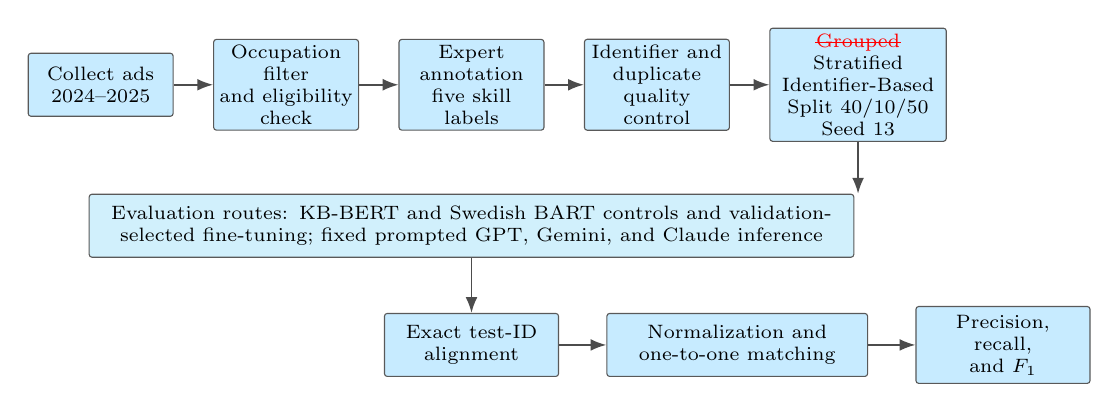
\begin{tikzpicture}[node distance=6mm and 5mm]
    \node[methodstage, text width=17mm, inner sep=2pt] (collect) {Collect ads\\2024--2025};
    \node[methodstage, text width=17mm, inner sep=2pt, right=of collect] (screen) {Occupation filter\\and eligibility check};
    \node[methodstage, text width=17mm, inner sep=2pt, right=of screen] (annotate) {Expert annotation\\five skill labels};
    \node[methodstage, text width=17mm, inner sep=2pt, right=of annotate] (qc) {Identifier and\\duplicate quality control};
    \node[methodstage, text width=21mm, inner sep=2pt, right=of qc] (split) {\OURSREV{Grouped}{Stratified Identifier-Based}\\Split 40/10/50\\Seed 13};

    \node[methodroute, text width=95mm, below=8mm of annotate] (routes) {Evaluation routes: KB-BERT and Swedish BART controls and validation-selected fine-tuning; fixed prompted GPT, Gemini, and Claude inference};
    \node[methodstage, text width=20mm, below=7mm of routes] (align) {Exact test-ID\\alignment};
    \node[methodstage, text width=31mm, right=6mm of align] (match) {Normalization and\\one-to-one matching};
    \node[methodstage, text width=20mm, right=6mm of match] (score) {Precision, recall,\\and $F_1$};

    \foreach \a/\b in {collect/screen,screen/annotate,annotate/qc,qc/split}
      \draw[methodarrow] (\a) -- (\b);
    \draw[methodarrow] (split.south) -- (split.south |- routes.north);
    \draw[methodarrow] (routes.south) -- (align.north);
    \draw[methodarrow] (align) -- (match);
    \draw[methodarrow] (match) -- (score);
  \end{tikzpicture}
  \caption{End-to-end study pipeline. \OURSREV{Grouped splitting}{Splitting by identifier} and exact identifier alignment prevent the same advertisement from being evaluated under incompatible partitions or test sets.}
  \label{fig:study-pipeline}
\end{figure}


\section{Results}
\label{results}

The results include four parts. The first part characterizes the contrasting profiles between the two job categories, which supports the reflection for RQ3. Section~\ref{subsec:before-after} answers RQ1 and RQ2 by comparing each supervised model with its task-unadapted control. Section~\ref{subsec:finetuned-vs-llm} sets the fine-tuned models against the prompted ones. Finally, Section~\ref{subsec:skill-type-results} breaks the comparison down by skill labels. Unless stated otherwise, we present every figure with macro boundary-relaxed containment $F_1$ computed as described in Section~\ref{keyapproaches}.

\subsection{Skill Profile Characteristics}
The annotation process revealed distinct and contrasting skill profiles across the two job categories, with certain skills being characteristic of journalists specifically. Following the initial definitions of different skill types in Section \ref{annotationscheme}, hard skills in software developers are identified as technical abilities and names of technologies such as ``PowerShell'', ``utveckling av lösningar baserade på SharePoint Online'' (developing solutions based on SharePoint Online), or ``Microsoft 365'' while soft skills in software developer job ads include, for example, ``kommunicera effektive'' (communicate effectively), ``god affärsförståelse'' (good business understanding), or ``talar och förstår svenska'' (speak and understand Swedish). Meanwhile, hard skills in journalists consist of personal qualities or traits which are necessary to produce measurable results in terms of audience engagement for the employer, for instance, ``starka kommunikationsfärdigheter på svenska och engelska i både tal och skrift'' (strong communication ability in Swedish and English in both speaking and writing), or ``snabbt kunna sätta dig in i nya frågor'' (quickly familiarize yourself with new topics). This study found that some hard skills in journalist job ads were actually categorized as soft skills in software developer job ads. Without the connection to journalistic work output, many of these journalistic hard skills would be defined as soft skills. This finding indicated that the distinction between skill types is not determined solely by the general definitions or the wording of a skill, yet, the distinction also depends on how the skill relates to the tasks, expected outputs, and broader context of the job. The two job categories in our study consequently exhibit contrasting skill profiles, illustrating how the meaning and classification of a skill can change across job category contexts.

%\RVNOTE{RQ3 rests on the claim that the two occupations have contrasting skill profiles, but no evidence is given here. Send, per occupation and per skill label, the total mentions, the mean mentions per advertisement, and the mean mention length in tokens, and the table and its paragraph can be drafted.} 

\begin{oursnewtext}
\RVNOTE{minh de danh phan nay va table \ref{tab:skill-profile} cho bai dataset nhe?} Table~\ref{tab:skill-profile} quantifies the occupational contrast in the corrected corpora. The journalist corpus contains more hard-skill, distinct-skill, and must-have mentions per advertisement, and those mentions are longer on average. For example, journalist hard skills average \OURSREV{15.02}{15.07} mentions per advertisement and \OURSREV{5.01}{4.99} whitespace-delimited tokens per mention, compared with 13.40 mentions and 2.79 tokens among software developers. Distinct skills show the largest length contrast, at 5.78 tokens for journalists and 2.11 for software developers. The direction reverses for soft skills and nice-to-have skills: software developer advertisements contain more of both per advertisement. The occupations therefore differ in both annotation density and surface realization; neither occupation is uniformly more skill-dense across all labels.
\end{oursnewtext}
\begin{table*}[width=\textwidth,pos=htbp]
  \centering
  \scriptsize
  \setlength{\tabcolsep}{3pt}
  \caption{\OURS{Skill profiles in the corrected annotated corpora. Mention length is the number of whitespace-delimited tokens after trimming; means include advertisements with zero mentions for the relevant label.}}
  \label{tab:skill-profile}
  \begin{tabular}{llrrrrr}
    \toprule
    \rowcolor{oursnewbg}Job category & Skill label & Advertisements & Mentions & Mean per ad & Mean tokens & Ads with at least one \\
    \midrule
    \rowcolor{oursnewbg}Software developers & Hard skills & 315 & 4,221 & 13.40 & 2.79 & 313 \\
    \rowcolor{oursnewbg}Software developers & Soft skills & 315 & 2,343 & 7.44 & 4.09 & 306 \\
    \rowcolor{oursnewbg}Software developers & Distinct skills & 315 & 179 & 0.57 & 2.11 & 83 \\
    \rowcolor{oursnewbg}Software developers & Must-have skills & 315 & \OURSREV{2,339}{2,291} & \OURSREV{7.43}{7.27} & \OURSREV{2.56}{2.62} & 286 \\
    \rowcolor{oursnewbg}Software developers & Nice-to-have skills & 315 & \OURSREV{927}{907} & \OURSREV{2.94}{2.88} & \OURSREV{2.01}{2.06} & 166 \\
    \midrule
    \rowcolor{oursnewbg}Journalists & Hard skills & 322 & \OURSREV{4,836}{4,853} & \OURSREV{15.02}{15.07} & \OURSREV{5.01}{4.99} & 321 \\
    \rowcolor{oursnewbg}Journalists & Soft skills & 322 & 1,825 & 5.67 & 2.90 & 283 \\
    \rowcolor{oursnewbg}Journalists & Distinct skills & 322 & 534 & 1.66 & 5.78 & 197 \\
    \rowcolor{oursnewbg}Journalists & Must-have skills & 322 & \OURSREV{7,012}{6,644} & \OURSREV{21.78}{20.63} & \OURSREV{4.35}{4.59} & 321 \\
    \rowcolor{oursnewbg}Journalists & Nice-to-have skills & 322 & \OURSREV{444}{434} & \OURSREV{1.38}{1.35} & \OURSREV{3.59}{3.67} & 177 \\
    \bottomrule
  \end{tabular}
\end{table*}


\subsection{Performance Before and After Fine-Tuning}
\label{subsec:before-after}

Table \ref{tab:overall-performance} shows an overall performance of each model under all three metrics. 
\begin{table}[pos=htbp]
  \centering
  \small
  \setlength{\tabcolsep}{4pt}
  \caption{Overall model performance. Values are unweighted means over all 18 job-category--skill-label cells under boundary-relaxed containment matching.}
  % [REV] Label renamed: \label{tab:before-after} was attached to three
  % different tables, so every \ref{tab:before-after} resolved to the last one.
  \label{tab:overall-performance}
  \begin{tabular}{llrrr}
    \toprule
    Model & Setting & Macro-Precision & Macro-Recall & Macro-F1 \\
    \midrule
    BERT & No fine-tune & \OURSREV{0.099}{0.095} & \OURSREV{0.544}{0.517} & \OURSREV{0.151}{0.144} \\
    BART & No fine-tune & \OURSREV{0.250}{0.277} & \OURSREV{0.037}{0.036} & \OURSREV{0.055}{0.056} \\
    BERT & Fine-tuned & \OURSREV{0.610}{0.588} & \OURSREV{0.722}{0.836} & \OURSREV{0.628}{0.659} \\
    BART & Fine-tuned & \OURSREV{0.629}{0.653} & \OURSREV{0.419}{0.455} & \OURSREV{0.462}{0.498} \\
    GPT & Prompted & \OURSREV{0.604}{0.601} & \OURSREV{0.699}{0.704} & \OURSREV{0.589}{0.590} \\
    Gemini & Prompted & \OURSREV{0.683}{0.680} & \OURSREV{0.653}{0.654} & \OURSREV{0.618}{0.619} \\
    Claude & Prompted & \OURSREV{0.656}{0.654} & \OURSREV{0.617}{0.630} & \OURSREV{0.591}{0.595} \\
    \bottomrule
  \end{tabular}
\end{table}




Table~\ref{tab:before-after} compares each supervised configuration with its task-unadapted control under the primary boundary-relaxed containment macro $F_1$. Each job category-level value is an unweighted mean over the six skill labels, with the adapted and unadapted configuration evaluated on identical test identifiers. Fine-tuning increased Swedish BERT score from \BertSoftwareBefore{} to \BertSoftwareAfter{} in software developers, from \BertJournalismBefore{} to \BertJournalismAfter{} in journalism, and from \BertMergedBefore{} to \BertMergedAfter{} in the merged setting. The corresponding absolute gains were respectively \BertSoftwareGain{}, \BertJournalismGain{}, and \BertMergedGain{}.
%\RVNOTE{Terminology pass, with the reasons. ``Software engineering'' becomes ``software developers'' because Section~\ref{method} samples and defines the category as software developers (\emph{systemutvecklare}) and every table is headed that way, so the Results were using a second name for the same group. ``Skill views'' becomes ``skill labels'' because the Annotation Scheme calls them labels, and ``view'' was pipeline vocabulary for the same five categories. The remaining ``skill view'' instances sit in comment lines of the auto-generated macro block and should be fixed in \texttt{sync\_latex\_results.py}.}

Swedish BART increased from \BartSoftwareBefore{} to \BartSoftwareAfter{} in software developers, from \BartJournalismBefore{} to \BartJournalismAfter{} in journalism, and from \BartMergedBefore{} to \BartMergedAfter{} in the merged setting. The corresponding gains were \BartSoftwareGain{}, \BartJournalismGain{}, and \BartMergedGain{}. The largest observed gain across the 36 fine-tuned configurations occurred for \LargestGainConfiguration{} (\LargestGainValue{}), while the smallest occurred for \SmallestGainConfiguration{} (\SmallestGainValue{}).

\begin{table}[H]
  \centering
  \small
  \setlength{\tabcolsep}{4pt}
  \caption{Performance before and after supervised fine-tuning. Scores are mean
  macro boundary-relaxed containment $F_1$ over six skill labels; each paired
  comparison uses identical test identifiers.}
  \label{tab:before-after}
  \begin{tabular}{llrrr}
    \toprule
    Model & Job category & Unadapted & Fine-tuned & Gain \\
    \midrule
    Swedish BERT & Software developers & \BertSoftwareBefore & \BertSoftwareAfter & \BertSoftwareGain \\
    Swedish BERT & Journalists & \BertJournalismBefore & \BertJournalismAfter & \BertJournalismGain \\
    Swedish BERT & Merged & \BertMergedBefore & \BertMergedAfter & \BertMergedGain \\
    \midrule
    Swedish BART & Software developers & \BartSoftwareBefore & \BartSoftwareAfter & \BartSoftwareGain \\
    Swedish BART & Journalists & \BartJournalismBefore & \BartJournalismAfter & \BartJournalismGain \\
    Swedish BART & Merged & \BartMergedBefore & \BartMergedAfter & \BartMergedGain \\
    \bottomrule
  \end{tabular}
\end{table}

The magnitude of a before--after difference has a different interpretation for the two model families. Swedish BERT control includes a newly initialized three-label head and therefore measures an untrained task interface. Swedish BART control retains a pretrained language-generation decoder but has not learned the study's skill serialization. Table~\ref{tab:before-after} demonstrates the value of task adaptation for each model but does not provide a symmetric comparison of two meaningful zero-shot extractors.

\subsection{Fine-Tuned Models and Prompted Large Language Models}
\label{subsec:finetuned-vs-llm}

Table~\ref{tab:cross-model-domain} compares the fine-tuned Swedish transformer-based models with the prompted GPT, Claude, and Gemini models after identifier alignment and common scoring. Under the primary metric, \BestSoftwareModel{} obtained the highest software developer score (\BestSoftwareScore{}), \BestJournalismModel{} obtained the highest journalist score (\BestJournalismScore{}) and the highest merged-domain score (\BestMergedScore{}). \begin{comment}\BestMergedModel{} obtained \end{comment}

\begin{table}[H]
  \centering
  \small
  \caption{Cross-model performance by job categories. Values are mean macro boundary-relaxed containment $F_1$ over six skill labels. Prompted systems use fixed model parameters at inference.}
  \label{tab:cross-model-domain}
  \begin{tabular}{lrrr}
    \toprule
    Model & Software developers & Journalists & Merged \\
    \midrule
    Fine-tuned Swedish BERT & \BertSoftwareScore & \BertJournalismScore & \BertMergedScore \\
    Fine-tuned Swedish BART & \BartSoftwareScore & \BartJournalismScore & \BartMergedScore \\
    Prompted GPT & \GptSoftwareScore & \GptJournalismScore & \GptMergedScore \\
    Prompted Claude & \ClaudeSoftwareScore & \ClaudeJournalismScore & \ClaudeMergedScore \\
    Prompted Gemini & \GeminiSoftwareScore & \GeminiJournalismScore & \GeminiMergedScore \\
    \bottomrule
  \end{tabular}
\end{table}

The best model for software developers had mean macro precision \BestSoftwarePrecision{} and recall \BestSoftwareRecall{}. The winner for journalists had precision \BestJournalismPrecision{} and recall \BestJournalismRecall{}, while the merged-domain winner had precision \BestMergedPrecision{} and recall \BestMergedRecall{}. Relative ranking therefore changed across job categories, namely prompted Gemini led among software developers whereas the source-bound fine-tuned BERT led in
journalists and the merged evaluation.

Across the five evaluated models and six skill labels, the mean increase from exact matching to boundary-relaxed containment matching was \SoftwareExactContainmentGap{} in software developers, \JournalismExactContainmentGap{} in journalists, and \MergedExactContainmentGap{} in the merged setting. The larger journalist difference indicates greater sensitivity to boundary extent or additional modifiers. The difference does not by itself establish semantic correctness because containment can also credit an overly broad phrase. Output-format compliance and unsupported-generation rate remain necessary diagnostics for BART and the prompted models.

\subsection{Performance across Skill Types}
\label{subsec:skill-type-results}

Table \ref{tab:by-skill-label} shows the mean scores following the five skill labels and the models while Table~\ref{tab:skill-winners} identifies the highest-scoring model in each job category--skill cell under the primary metric. %The table was generated directly from the verified result CSV rather than transcribed manually.

% [REV] Original placement was \begin{table}[H].
\begin{table}[pos=htbp]
  \centering
  \small
  \setlength{\tabcolsep}{4pt}
  \caption{Mean macro boundary-relaxed containment F1 by skill label. Values are unweighted means across software developers, journalists, and the merged setting.}
  \label{tab:by-skill-label}
  \begin{tabular}{llrrrr}
    \toprule
    Skill label & Fine-tuned BERT & Fine-tuned BART & GPT & Gemini & Claude \\
    \midrule
    Hard skills & \OURSREV{0.717}{0.706} & \OURSREV{0.502}{0.514} & \OURSREV{0.556}{0.566} & \OURSREV{0.575}{0.582} & \OURSREV{0.571}{0.577} \\
    Soft skills & \OURSREV{0.712}{0.726} & \OURSREV{0.541}{0.637} & \OURSREV{0.607}{0.616} & \OURSREV{0.671}{0.679} & \OURSREV{0.638}{0.651} \\
    Distinct skills & \OURSREV{0.325}{0.466} & \OURSREV{0.304}{0.320} & \OURSREV{0.438}{0.430} & \OURSREV{0.420}{0.422} & \OURSREV{0.355}{0.372} \\
    Must-have skills & \OURSREV{0.652}{0.667} & \OURSREV{0.451}{0.499} & \OURSREV{0.437}{0.453} & \OURSREV{0.532}{0.542} & \OURSREV{0.517}{0.518} \\
    Nice-to-have skills & \OURSREV{0.593}{0.616} & \OURSREV{0.458}{0.446} & 0.804 & \OURSREV{0.810}{0.819} & \OURSREV{0.775}{0.799} \\
    All skills & \OURSREV{0.768}{0.776} & \OURSREV{0.516}{0.569} & \OURSREV{0.693}{0.670} & \OURSREV{0.702}{0.670} & \OURSREV{0.690}{0.656} \\
    \bottomrule
  \end{tabular}
\end{table}

\begin{table}[H]
  \centering
  \small
  \caption{Best model by job category and skill label under boundary-relaxed containment macro $F_1$.}
  \label{tab:skill-winners}
  \begin{tabular}{llll}
    \toprule
    Skill label & Software developers & Journalists & Merged \\
    \midrule
    \SkillWinnerRows
    \bottomrule
  \end{tabular}
\end{table}

Fine-tuned Swedish BERT led \OURSREV{11}{13} of the 18 job category--skill cells: every all-skills, hard-skills, and soft-skills evaluation, as well as \OURSREV{}{distinct-skill and }must-have extraction in journalists and the merged setting. Prompted models led the remaining \OURSREV{seven}{five} cells. \OURSREV{GPT led distinct-skill extraction in journalists and the merged setting.}{GPT did not lead an individual cell.} Gemini led software developer distinct and must-have extraction and journalist and merged nice-to-have extraction. Claude led software developer nice-to-have extraction. Swedish BART did not lead an individual cell under the primary metric. These counts describe the evaluated models but do not establish an architecture-family ordering.

The distribution of winners suggests a difference between content-oriented and status-oriented views. Fine-tuned BERT consistently led the broad all-skills view and both principal content categories, which is consistent with source-bound supervision being effective for recurring hard- and soft-skill mentions. Prompted models were more competitive for distinct and nice-to-have skills. Sparse labels, occupational judgment, and long-range requirement cues are proper explanations, but the present results do not isolate their causal contribution. Skill-type difficulty cannot be inferred from $F_1$ alone. Simultaneously, annotation density, exact agreement, mention length, precision--recall balance, and fine-tuning gain must also be considered.


\section{Discussion}
\label{discussions}

This study explores the current performance of language models on skill extraction for Swedish job ads. Namely, we formulated three specific questions including how well existing Swedish transformer-based models and prompted commercial LLMs extract skills from Swedish job ads without domain-specific adaptation (RQ1), how much supervised fine-tuning on expert-annotated Swedish data changes that picture (RQ2), and whether the relative standing of the fine-tuned regimes depends on the job categories (RQ3). Three findings organize the interpretation below. First, neither Swedish reference checkpoint produces usable extractions before adaptation, whereas the prompted systems produce competitive output from a written instruction alone. Second, fine-tuning on a few hundred expert-annotated Swedish job ads moves the encoder-only BERT from a near-zero score to the level of the strongest prompted system. Third, the ordering of the two regimes is not stable because this ordering reverses between software developer and journalist job ads, and it varies further across the five annotated skill labels. Taken together, the choice between a fine-tuned Swedish model and a prompted commercial model is not one decision but a decision conditioned on job categories and on the kind of skill being sought.


\subsection{Positioning Relative to Prior Work}

Prior work establishes BERT-style sequence labeling as a strong and common skill-extraction formulation \citep{zhang2022skillspan,senger2024survey}, while generative NER shows that extraction can instead be represented as  conditional text generation \citep{yan2021generative,cui2021template}. Prompt-based LLM studies add a third adaptation regime in which task behavior is elicited without supervised parameter updates  \citep{nguyen2024rethinking}. Multilingual and multidomain evaluations further show why findings from one language or document type should not be assumed to transfer unchanged \citep{vasquezrodriguez2026multilingual}. The present study sits at the intersection of these three lines and asks whether their relative behavior holds for Swedish.

To the best of our knowledge, this is the first study to benchmark Swedish skill extraction across supervised and prompted regimes on job ads annotated by domain experts. The closest Swedish precedent annotated 260 job ads with general annotators across occupations that were not explicitly specified, and fine-tuned a Swedish encoder for skills alongside other entity types \citep{stollenwerk2023annotated}. Our design differs in four respects that are particularly relevant to the labor-market questions these data are intended to address including annotation by experts in the two job categories concerned; a label set that separates what a skill is (hard, soft, distinct) from how strongly it is required (must-have, nice-to-have); two deliberately contrasting job categories rather than a mixed pool; and a single scoring pipeline applied to a fine-tuned encoder, a fine-tuned encoder--decoder, and three commercial LLMs on identical test identifiers. Being first is a limitation as much as a contribution. There is no external Swedish benchmark against which our absolute numbers can be calibrated, so the values reported here should be read as an initial reference point that subsequent Swedish work is expected to revise rather than as established performance levels for the language.

\subsection{Interpreting the Performance Patterns}

\paragraph{Fine-tuning gains and what they do not show.} Fine-tuning raised boundary-relaxed containment macro $F_1$ by \BertSoftwareGain{} to \BertMergedGain{} for the encoder-only model and by \BartJournalismGain{} to \BartMergedGain{} for the encoder--decoder model, depending on the setting. These are the largest single effects in the study, however, as Section~\ref{subsec:before-after} sets out, their magnitude is partly a property of the two controls rather than of the models themselves. The defensible reading is narrower than the numbers suggest: with roughly 40 percent of a few hundred job ads available for training, both Swedish checkpoints learn the annotation scheme well enough to reach a usable operating point, and the encoder-only formulation learns it more efficiently than the generative one.

\paragraph{Source-bound labeling versus free generation.} The fine-tuned encoder-only model scored \BertSoftwareScore{},
\BertJournalismScore{}, and \BertMergedScore{} across the three settings, against \BartSoftwareScore{}, \BartJournalismScore{}, and \BartMergedScore{} for the fine-tuned encoder--decoder, and the latter did not lead a single job category--skill cell. The two formulations differ in what they have to learn. The encoder-only model assigns a label to tokens that already exist in the job ad. Thus, this encoder-only model's output is bounded by the source text and it never has to learn how to spell or delimit a skill. The encoder--decoder model must generate the skill list as free text, so it learns what to extract, how to render it, and how to separate items, all from the same small training signal. The larger hypothesis space is an asset when gold annotations are paraphrases or discontinuous expressions that flat BIO tagging cannot represent, but this space is a liability at this data scale. This should be read as a  statement about these two Swedish checkpoints under these training budgets, and not as an ordering of encoder-only and encoder--decoder architectures in general.

\paragraph{The domain reversal.} Prompted Gemini obtained the highest software developer score (\GeminiSoftwareScore{}) ahead of the fine-tuned encoder BERT (\BertSoftwareScore{}), while the fine-tuned encoder BERT led among journalists (\BertJournalismScore{} against the result of Gemini \GeminiJournalismScore{}) and in the merged setting (\BertMergedScore{} against the result of Gemini \GeminiMergedScore{}). A reasonable reading follows from how the two job categories write about skills. Skills in software developer job ads are dominated by named technologies, tools, frameworks, and abbreviations that are short, largely language-independent, and abundantly represented in the pretraining data of large commercial models. Recognizing \emph{Kubernetes} or \emph{CI/CD} inside a Swedish sentence requires little
Swedish and no exposure to our annotation scheme. Journalist job ads express a larger share of skills as longer Swedish phrases whose extent is a matter of convention rather than of vocabulary. What has to be learned is precisely the annotation convention, which supervised fine-tuning supplies and
a prompt does not. RQ3 is therefore answered affirmatively, and with a methodological consequence: a Swedish benchmark built on technology-dense job ads alone would have produced the opposite recommendation to one built on journalist job ads.

\paragraph{Skill type matters more than the aggregate means.}
The fine-tuned encoder BERT led \OURSREV{11}{13} of the 18 job category--skill cells, yet it did not lead the software developer mean, because that mean is pulled down by the \OURSREV{views}{skill-label settings} in which it is weakest. \OURSREV{Prompted models led the remaining seven cells in a patterned way, concentrated on distinct skills and nice-to-have skills.}{Prompted models led the remaining five cells, with four wins achieved on distinct or nice-to-have skills and one win secured on a software-developer must-have skill.} Requirement-status labels are marked in Swedish job ads by a small and largely closed set of lexical triggers such as \emph{meriterande}, \emph{önskvärt}, \emph{krav}, and \emph{krävs}. This is a cue that can be stated completely in a prompt, and the nice-to-have cells carry the highest scores compared to the other skill labels in the study (\NiceToHaveLow{} to \NiceToHaveHigh{}). Conversely, distinct skills behave in the opposite way. This is the lowest-scoring label in every setting (\DistinctLow{} to \DistinctHigh{}) and also the label on which our own domain experts agreed least, with exact agreement of \AgreeExactLow{} and containment agreement of \AgreeContainLow{} among journalists. The definition of the distinct skills—skills that are not typical of the job—requires a judgment about the occupation as a whole rather than a decision about the text at hand. The low scores on this label therefore measure definitional difficulty at least as much as model capability, which is an argument for reporting skill labels separately rather than only in
aggregate.

\paragraph{Boundary extent rather than skill identification.} Moving from exact string matching to boundary-relaxed containment increased the measured gap by \SoftwareExactContainmentGap{} among software developers, \JournalismExactContainmentGap{} among journalists, and \MergedExactContainmentGap{} in the merged setting. The same pattern is present in the human annotations, where exact agreement ranged from \AgreeExactLow{} to \AgreeExactHigh{} while containment agreement ranged from \AgreeContainLow{} to \AgreeContainHigh{}. The gap is therefore not an artifact of applying a lenient metric to machine output. Domain experts working from the same guideline disagree about the boundaries of skill phrases roughly as often as the models do, while agreeing on which skill is present. Two implications follow. First, exact match alone understates achievable performance on this task and should not be shown in isolation. Second, the containment agreement band of the annotators provides an informal reference point for the performance that a Swedish skill extractor can be expected to achieve. Against this reference, our best models with scores ranging from \BestJournalismScore{} to \BestSoftwareScore{} are approaching but have not entered the human consistency range. The two quantities are not strictly comparable, since agreement was computed as micro $F_1$ over the overlap sample while model scores are macro averages over job ads. Hence, the comparison should be interpreted as an order-of-magnitude reference rather than as a formal performance.

\subsection{Implications for Method}
The study shows that methodological choices in fine-tuning have to take job category-specific characteristics into account when annotation is prepared for skill extraction from job ad datasets. Definition of skill types may differ between job categories, which requires use of delimitations relevant for each category. Job-specific traditions in how job ads are presented may also need to be taken into account. The example of more complex presentations of journalist jobs, versus more concise bullet-point style presentations of skill requirements for software developer jobs, implies advantages of using text-type specific extraction and classification approaches.

Three further methodological points follow from the results. First, agreement and performance should both be reported at more than one strictness level. Reporting exact match alone would have made this task look considerably harder than it is, while reporting relaxed matching alone would have concealed a real and interpretable source of error. Second, the label set is itself an experimental variable rather than a neutral  container. Specifically, the label on which our domain experts agreed least is also the label on which every model scored lowest, so label design and model evaluation cannot be treated as independent steps. Third, a shared normalization and one-to-one matching pipeline applied to identical test identifiers is a precondition for comparing models whose outputs are not natively commensurable, because a source-bound tagger, a generative model, and a prompted API return objects of different kinds.

\subsection{Implications for Practice}

The operating point matters more for practice than the ranking does. The best models recovered roughly two thirds of the expert-annotated skills at an acceptable boundary. That level is not adequate for decisions about an individual applicant or an individual vacancy, where a missed requirement has a direct consequence for a person. It is informative for aggregate analysis, such as skill-demand monitoring, curriculum planning, and regional or temporal comparison, where errors on single job ads partly cancel across large volumes. A realistic near-term deployment is therefore assisted annotation, in which the model supplies a first pass that a domain expert corrects, rather than unattended automation.

For organizations choosing an approach, our results support a conditional recommendation. Where the target occupation is technology-dense and no annotated data exists, a prompted commercial model is a defensible starting point and requires no annotation budget. Where skills are expressed as longer contextual phrases, as in the journalist job ads, investment in expert annotation pays off, and a few hundred annotated job ads proved sufficient to overtake the prompted models.

In public sector settings, accuracy is not the only consideration when choosing a model. Locally fine-tuned Swedish models offer several practical advantages. They can be versioned and re-run consistently, operated at predictable cost on local hardware, and kept within an organization’s own infrastructure. This is particularly important when job ads or applicant data are subject to data protection regulations. By contrast, prompted commercial models are updated by their providers on schedules that technicians cannot control. As a result, a labor-market time series based on a commercial model may change over time because the model itself has changed, rather than because the labor market has changed. Thus, for a national agency, such as Arbetsförmedlingen, this provides a strong practical reason to prefer a local model even when its accuracy is only comparable to that of a commercial alternative.


\subsection{Implications for Research}
% [REV] New content.

The approach developed here is deliberately modular, consisting of an annotation scheme, a surface-alignment step, a fine-tuning stage, a shared normalization step, and a graded matching cascade. Only the annotation scheme is specific to skills while the other components do not depend on the type of information being extracted. This makes the overall approach general rather than specific to this study. Hence, the same pipeline can be adapted to other types of information in job ads by changing the labels and annotation guidelines. Other possible applications can be, for example, educational requirements, certifications, contract types, work locations, and language requirements. This flexibility is a key reason to establish a first Swedish benchmark. This signifies that once the annotation and evaluation infrastructure has been developed, it can be reused for other information-extraction tasks.

The evaluation approach is also independent of the models. Since the evaluation compares normalized sets of extracted strings using fixed test identifiers, new models can be added, evaluated, and compared with the results reported here without requiring new annotation. This means that the benchmark can remain useful even as the individual models included in this study become outdated. This is particularly valuable given how quickly commercial models are updated and replaced.

\subsection{Limitations}
\label{subsec:limitations}

Several limitations qualify the findings. The corpus is modest, comprising 315 software developer and 322 journalist job ads drawn from two job categories. Thus, the results characterize those two job categories rather than the Swedish labor market as a whole. All reported model results arise from a single data and training seed and a single stratified split, so standard deviations across seeds and confidence intervals over training randomness are unavailable. At the same time, differences of a few points between models should not be treated as established. Paired bootstrap intervals over test job ads would quantify test-sample uncertainty without retraining, but would not measure optimization variance.

The prompted models are zero-shot in prompt format but not label-free in development because the automated prompt-optimization stage used annotated development examples and the resulting prompts were then revised manually. The prompted models are consequently not a pure no-supervision baseline, and RQ2 should be explained accordingly. Commercial models may be updated by their providers, so the prompted results are tied to the model versions and access period described in Section~\ref{LLMMethod}. 

Additionally, the training setup for the transformer-based models also has some limitations. For the encoder-only model, since the dataset stores skill strings rather than gold character offsets, the token-level supervision for the encoder-only model is weakly aligned. Namely, an annotated paraphrase that does not occur verbatim in the text supplies no supervision. \OURSREV{Meanwhile, the limitation of the encoder--decoder model is different. When a job ad is divided into chunks, each chunk is paired with the full list of skills annotated for the entire job ad. As a result, a chunk may be trained to predict skills that do not actually appear in that chunk. Thus, the matching cascade is greedy in prediction order rather than a globally optimal bipartite assignment.}{Each BART skill is assigned to chunks containing its normalized contiguous token sequence, with a deterministic greatest-token-overlap fallback applied when no chunk contains the skill. Evaluation utilizes deterministic maximum-cardinality bipartite matching separately at each cascade level rather than relying on greedy prediction order.}

Finally, the comparison should be understood as a comparison of different model and task configurations and adaptation strategies, rather than as a comparison of model architectures. The supervised models are trained on annotated data and use different output formats, while the commercial LLMs generate their outputs directly from prompts. The encoder-only control uses an untrained classification head. All the models are evaluated using the same normalization and matching pipeline and the identical advertisement identifiers, which makes their outputs comparable for scoring. However, consistent scoring does not eliminate the underlying differences in supervision, output constraints, and model access. The findings should therefore be interpreted only for the Swedish checkpoints, prompts, occupations, skill labels, and data split evaluated in this study.


%\RVNOTE{The figures quoted in this section now come from macros, but those eight macros are maintained by hand in the preamble rather than emitted by \texttt{sync\_latex\_results.py}. Adding them to that script would close the last route by which this section can go stale.}


\section{Conclusions}
\label{conclusions}

%\RVNOTE{Please check that the three contributions are phrased as in the introduction, and confirm the release claim once the repository exists.}

This paper evaluated transformer-based and large language models for skill extraction for Swedish job ads in two job categories with contrasting skill profiles including software developers and journalists, using corpora annotated by experts in each field under five skill labels.

None of Swedish transformer-based models extracts skills usefully without task-specific adaptation whereas the prompted commercial models produce competitive output from instructions alone. Fine-tuning on a few hundred expert-annotated job ads substantially improves the performance. Namely, in the merged setting, boundary-relaxed containment macro $F_1$ increased from \BertMergedBefore{} to \BertMergedAfter{} for the Swedish encoder-only model and from \BartMergedBefore{} to \BartMergedAfter{} for the Swedish encoder--decoder model. This makes the encoder-only model reach the performance level of the strongest prompted model. However, the ranking of these two models is not stable across job categories. Specifically, while a prompted model obtained the highest score for software developers (\BestSoftwareScore{}), the fine-tuned Swedish encoder model performed best for journalists (\BestJournalismScore{}) and in the merged evaluation (\BestMergedScore{}). Moreover, performance also varies across skill labels. Several residual error concerns involve where a skill phrase begins and ends rather than which skill is present.

The study makes the three primary contributions. Our study provides the first benchmark of Swedish skill extraction spanning fine-tuned and prompted language models on expert-annotated data. We quantify the gain from fine-tuning relative to prompting, separately for each job category and each skill label. Finally, we release annotated Swedish corpora for software developer and journalist job ads.

The key finding is that the better adaptation regime depends on how skills are described in a job ad rather than from the model itself. When skills appear as short named technologies, a general model that has already encountered those names during pretraining performs well without any Swedish task-specific annotation. For where skills appear as longer phrases whose extent is set by convention and the convention has to be learned from annotated examples, supervised fine-tuning shows good performance. This has a practical implication for organizations working with Swedish labor-market job ads. A locally fine-tuned Swedish model as our fine-tuned models in this study becomes competitive with commercial systems at a few hundred annotated job ads. The models can be run consistently at a later date and securely operated inside an organization's own infrastructure when data protection becomes significant at present. Given the accuracy levels shown in this study, the appropriate use of these models is aggregate analysis and assisted annotation rather than unattended decisions about individual applicants or job vacancies.


\subsection{Future Research}

We propose four directions for future research based on this work. First, extraction is the first step in a longer pipeline, so linking extracted mentions to a taxonomy such as ESCO or SSYK is a separate task \citep{decorte2022design,desanto2026skillens}. The normalization used here aims for evaluation and does not perform for taxonomy linking. Hence, adding a linking step would allow to use Swedish skill mentions in statistics that can be compared across countries. Second, our formulation currently covers explicit mentions only, whereas implicit skills remain out of scope as clarified in Section \ref{bg:skillextraction}. The finding that some hard skills in journalists can only be identified through their connection to a measurable work output suggests that the distinction between explicit and implicit skills may depend on the job itself and therefore requires further study. Third, our current flat BIO tagging works well for most straightforward skill mentions but cannot easily represent nested, overlapping, or discontinuous mentions. Since a substantial number of the residual error are boundary-related, span-based and set-generation formulations with copy constraints naturally become a next step for this research task in Swedish. Finally, the approach could be extended to other Scandinavian languages due to the closeness between these languages. The annotation scheme and process developed in this study can conceptually be adapted to Norweigian or Danish job ads, allowing future work to examine whether the domain effects observed in this study are specific to Swedish or reflect a broader language-independent pattern.


\section*{Data availability}
% [REV] New section. Contribution (3) in the Introduction promises to release
% the annotated datasets, and most journals in this area now require a
% statement of this kind.
\begin{revnewtext}
The annotated Swedish job advertisement datasets for the software developer and
journalist categories, the annotation guideline, and the fifteen final prompts
are released with this article. The underlying advertisements are public
records published by Arbetsförmedlingen; the released files add the expert skill
annotations under the five labels described in Section~\ref{method}.
\end{revnewtext}
\RVNOTE{Insert the repository DOI or URL, the licence, and, if the raw
advertisement text cannot be redistributed, say which fields are released and
how the originals can be retrieved. The journal will also want a declaration of
competing interests and a funding statement here.}

\appendix

\section{Annotation Criteria}
\label{app:annotation}

\begin{center}
    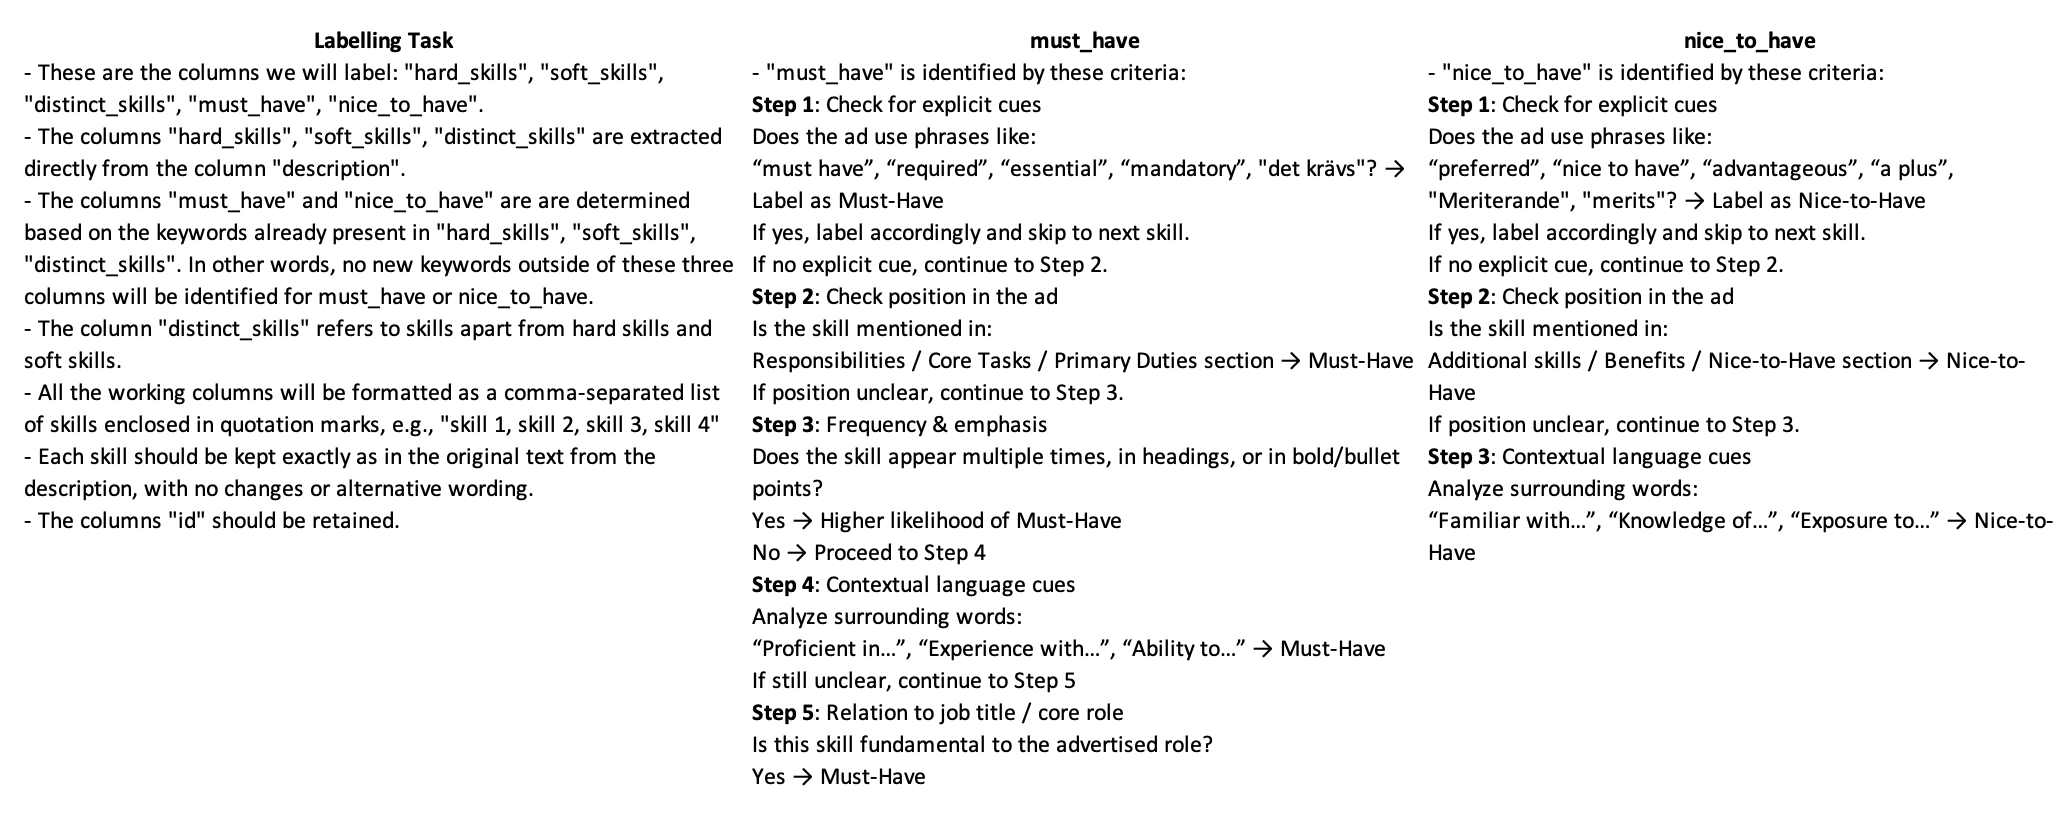
\includegraphics[width=\textwidth]{figs/annotationcriteria.png}
    
    \textbf{Figure A1:} Detailed annotation criteria.
\end{center}

\section{Final Prompts}
\label{app:prompts}
\RVNOTE{Paste the fifteen final prompts, one per skill label and model, as
produced by the Metagente optimization and then revised by hand
(Section~\ref{subsubsec:prompt-generation}). Verbatim listings are appropriate
here so that reviewers can reproduce the prompted runs.}


\section*{Declaration of competing interest}
\OURS{The authors declare that they have no known competing financial interests or personal relationships that could have appeared to influence the work reported in this paper.}


\section*{Funding}
\OURS{[AUTHOR TO INSERT THE FUNDER AND GRANT NUMBER, OR STATE THAT THIS RESEARCH RECEIVED NO SPECIFIC GRANT FROM FUNDING AGENCIES IN THE PUBLIC, COMMERCIAL, OR NOT-FOR-PROFIT SECTORS.]}

\section*{Declaration of generative AI use}
\OURS{During preparation of this work, the authors used generative AI tools for language editing and code assistance. The authors reviewed and edited all affected material and take full responsibility for the content of the publication.}
% [REV] cas-sc boilerplate appendix, kept for reference:
% \section{My Appendix}
% Appendix sections are coded under \verb+\appendix+.
% \verb+\printcredits+ command is used after appendix sections to list
% author credit taxonomy contribution roles tagged using \verb+\credit+
% in frontmatter.

\printcredits

%% Loading bibliography style file
% \bibliographystyle{model1-num-names}
\bibliographystyle{cas-model2-names}

% Loading bibliography database
\bibliography{cas-refs}



\end{document}
